\chapter{Experimental Evaluation}
\label{ch:evaluation}

\section{Experimental Setup}
\label{sec:eval_setup}

\subsection{Hardware, Software, and Datasets}
\label{subsec:eval_hardware}

All experiments were conducted on a single workstation (Intel Core i7-8850H,
32\,GB DDR4, CPU-only execution, Ubuntu 22.04 LTS, Python~3.12, PyTorch~2.x).
Unless otherwise noted, tables report the benchmark run whose configuration
(seed, duration, hyperparameters) is stated alongside the result.

The evaluation combines three datasets because the framework has three claims:
edge-node detection accuracy, topology-aware RCA, and coordinator scalability.
The \textbf{Server Machine Dataset (SMD)}~\cite{su2019robust}, hosted by
Tsinghua University, is a standard AIOps benchmark with dense multivariate
metrics from 28~machines and human-verified anomaly labels; it isolates the
LSTM-AE detector and DP analysis from trace-topology effects.
\textbf{Train-Ticket} provides a realistic ticket-booking microservice topology
for RCA evaluation; this thesis uses an 11-service topology slice and
trace-style fault propagation, consistent with distributed-trace RCA work
\cite{zhang2019rootcause, zhang2019tracing}, to measure Top-1/Top-3 and MRR
against known injected faults. \textbf{Alibaba Cluster Trace}~\cite{alibaba2022cluster} provides large-scale production traces used to
derive node-count and connection-density scenarios for coordinator scalability,
aggregation latency, memory growth, and adaptive compression.

Table~\ref{tab:topology_summary} summarizes the two RCA evaluation topologies.
The Train-Ticket topology is a direct 11-service slice of the open-source
ticket-booking benchmark. The Alibaba-derived topology is a \emph{synthetic}
graph constructed from the degree distribution and call-depth statistics of
Alibaba cluster-001 traces: 50~services were sampled with a maximum call depth
of~6, producing 112~directed edges, and the same three fault types (latency
spike, CPU overload, cascade failure) were injected programmatically.

\begin{table}[H]
    \centering
    \small
    \begin{tabular}{|l|c|c|l|}
        \hline
        \textbf{Topology} & \textbf{Services} & \textbf{Edges}
        & \textbf{Fault types injected} \\
        \hline
        Train-Ticket & 11 & 19 & latency spike, CPU overload, cascade \\
        \hline
        Alibaba (derived) & 50 & 112 & same 3 types; sampled from \\
        & & & cluster-001, max depth~=~6 \\
        \hline
    \end{tabular}
    \caption{RCA evaluation topologies. The Alibaba topology is a synthetic
             graph built from Alibaba's published degree distribution, not a
             direct trace replay.}
    \label{tab:topology_summary}
\end{table}

The evaluation uses the full 38-channel SMD input as a $(50 \times 38)$
normalized window, matching the telemetry pipeline in
Section~\ref{sec:metrics_collection}.

\subsection{Baselines and Evaluation Metrics}
\label{subsec:eval_baselines}

Five baselines are compared: (1)~a \textbf{static 3$\sigma$} untrained
LSTM-AE; (2)~a \textbf{centralized LSTM-AE} trained without FL or DP;
(3)~the proposed \textbf{federated LSTM-AE} with FedAvg;
(4)~\textbf{EWMA} thresholding ($\alpha = 0.05$); and
(5)~\textbf{random RCA} (uniform root cause selection). Detection quality
uses F1, AUC-ROC, AUC-PR, and inference latency. Privacy sweeps $\sigma$
and $C$; communication reports payload size and compression cost; RCA uses
Top-1, Top-3, and MRR; thresholding uses alert count, FPR, and reward;
scalability uses aggregation latency and coordinator memory.

\textbf{Reproducibility and statistical reporting.} Each reported result is
taken from the benchmark run whose configuration is stated in the corresponding
table or figure caption. The protocol is reproducible from the logged settings:
SMD windows use $L=50$ and $F=38$, Config~C uses $h=128$, two LSTM layers,
learning rate $10^{-3}$, and seed~42; DP experiments run for 200 rounds; RCA
logs 100 Train-Ticket and 50 Alibaba events; and thresholding logs a
10\,020-minute SMD reconstruction-error stream. RCA accuracy is interpreted
with Wilson 95\% confidence intervals, and FL latency is summarized over the
10~logged rounds. To quantify seed sensitivity, the LSTM-AE (Config~C) was
retrained with three seeds (42, 123, 7); results are reported in
Table~\ref{tab:detection_results} and discussed in
\S\ref{sec:eval_detection}.

% ============================================================================
\section{Anomaly Detection Performance}
\label{sec:eval_detection}

\begin{table}[H]
    \centering
    \small
    \begin{tabular}{|l|c|c|c|c|c|c|}
        \hline
        \textbf{Model} & \textbf{Prec.} & \textbf{Rec.} & \textbf{F1}
        & \textbf{AUC-ROC} & \textbf{AUC-PR} & \textbf{Lat.\,(ms)} \\
        \hline
        Static 3$\sigma$ & 0.000 & 0.000 & 0.000 & 0.372 & 0.157 & 0.24 \\
        \hline
        Centralized LSTM-AE & 0.664 & 0.396 & 0.496 & 0.888 & 0.655 & 0.21 \\
        \hline
        Federated LSTM-AE & \textbf{0.813} & \textbf{0.868} & \textbf{0.839}
        & \textbf{0.950} & \textbf{0.895} & 0.21 \\
        \hline
    \end{tabular}
    \caption{Detection performance on SMD (Config~C, 100 epochs). The
             primary result is from the pre-trained checkpoint (seed~42).
             A 3-seed retraining (seeds 42, 123, 7) yields
             F1~$= 0.743 \pm 0.077$ and
             AUC-ROC~$= 0.932 \pm 0.017$,
             confirming that AUC-ROC is stable while F1 is
             sensitive to threshold calibration.}
    \label{tab:detection_results}
\end{table}

The federated LSTM-AE ($h{=}128$, $L{=}2$, $\text{lr}{=}0.001$, seed~42)
achieves F1~$=$~0.839 and AUC-ROC~$=$~0.950, substantially outperforming the
centralized baseline (F1~$=$~0.496). The static 3$\sigma$ baseline fails
entirely (F1~$=$~0.0), confirming that a fixed threshold on an untrained model
is inadequate for multivariate telemetry.

\textbf{Multi-seed variance.} Retraining Config~C with three seeds (42, 123,
7) produces F1 values of 0.661, 0.846, and 0.721
(mean $0.743 \pm 0.077$), while AUC-ROC remains stable at
$0.932 \pm 0.017$ (range 0.911--0.954). The F1 variance is driven by recall
sensitivity to the 95th-percentile threshold: small shifts in the
reconstruction-error distribution change which windows cross the threshold.
AUC-ROC, being threshold-independent, provides a more robust performance
estimate.

To contextualize these results, OmniAnomaly~\cite{su2019robust}---the paper
that introduced SMD---reports F1~$\approx$~0.83 on a subset of SMD machines.
The federated LSTM-AE is therefore competitive with a published
state-of-the-art detector, while operating without centralizing raw telemetry.
This comparison uses the authors' reported numbers rather than a re-run.

\begin{figure}[H]
    \centering
    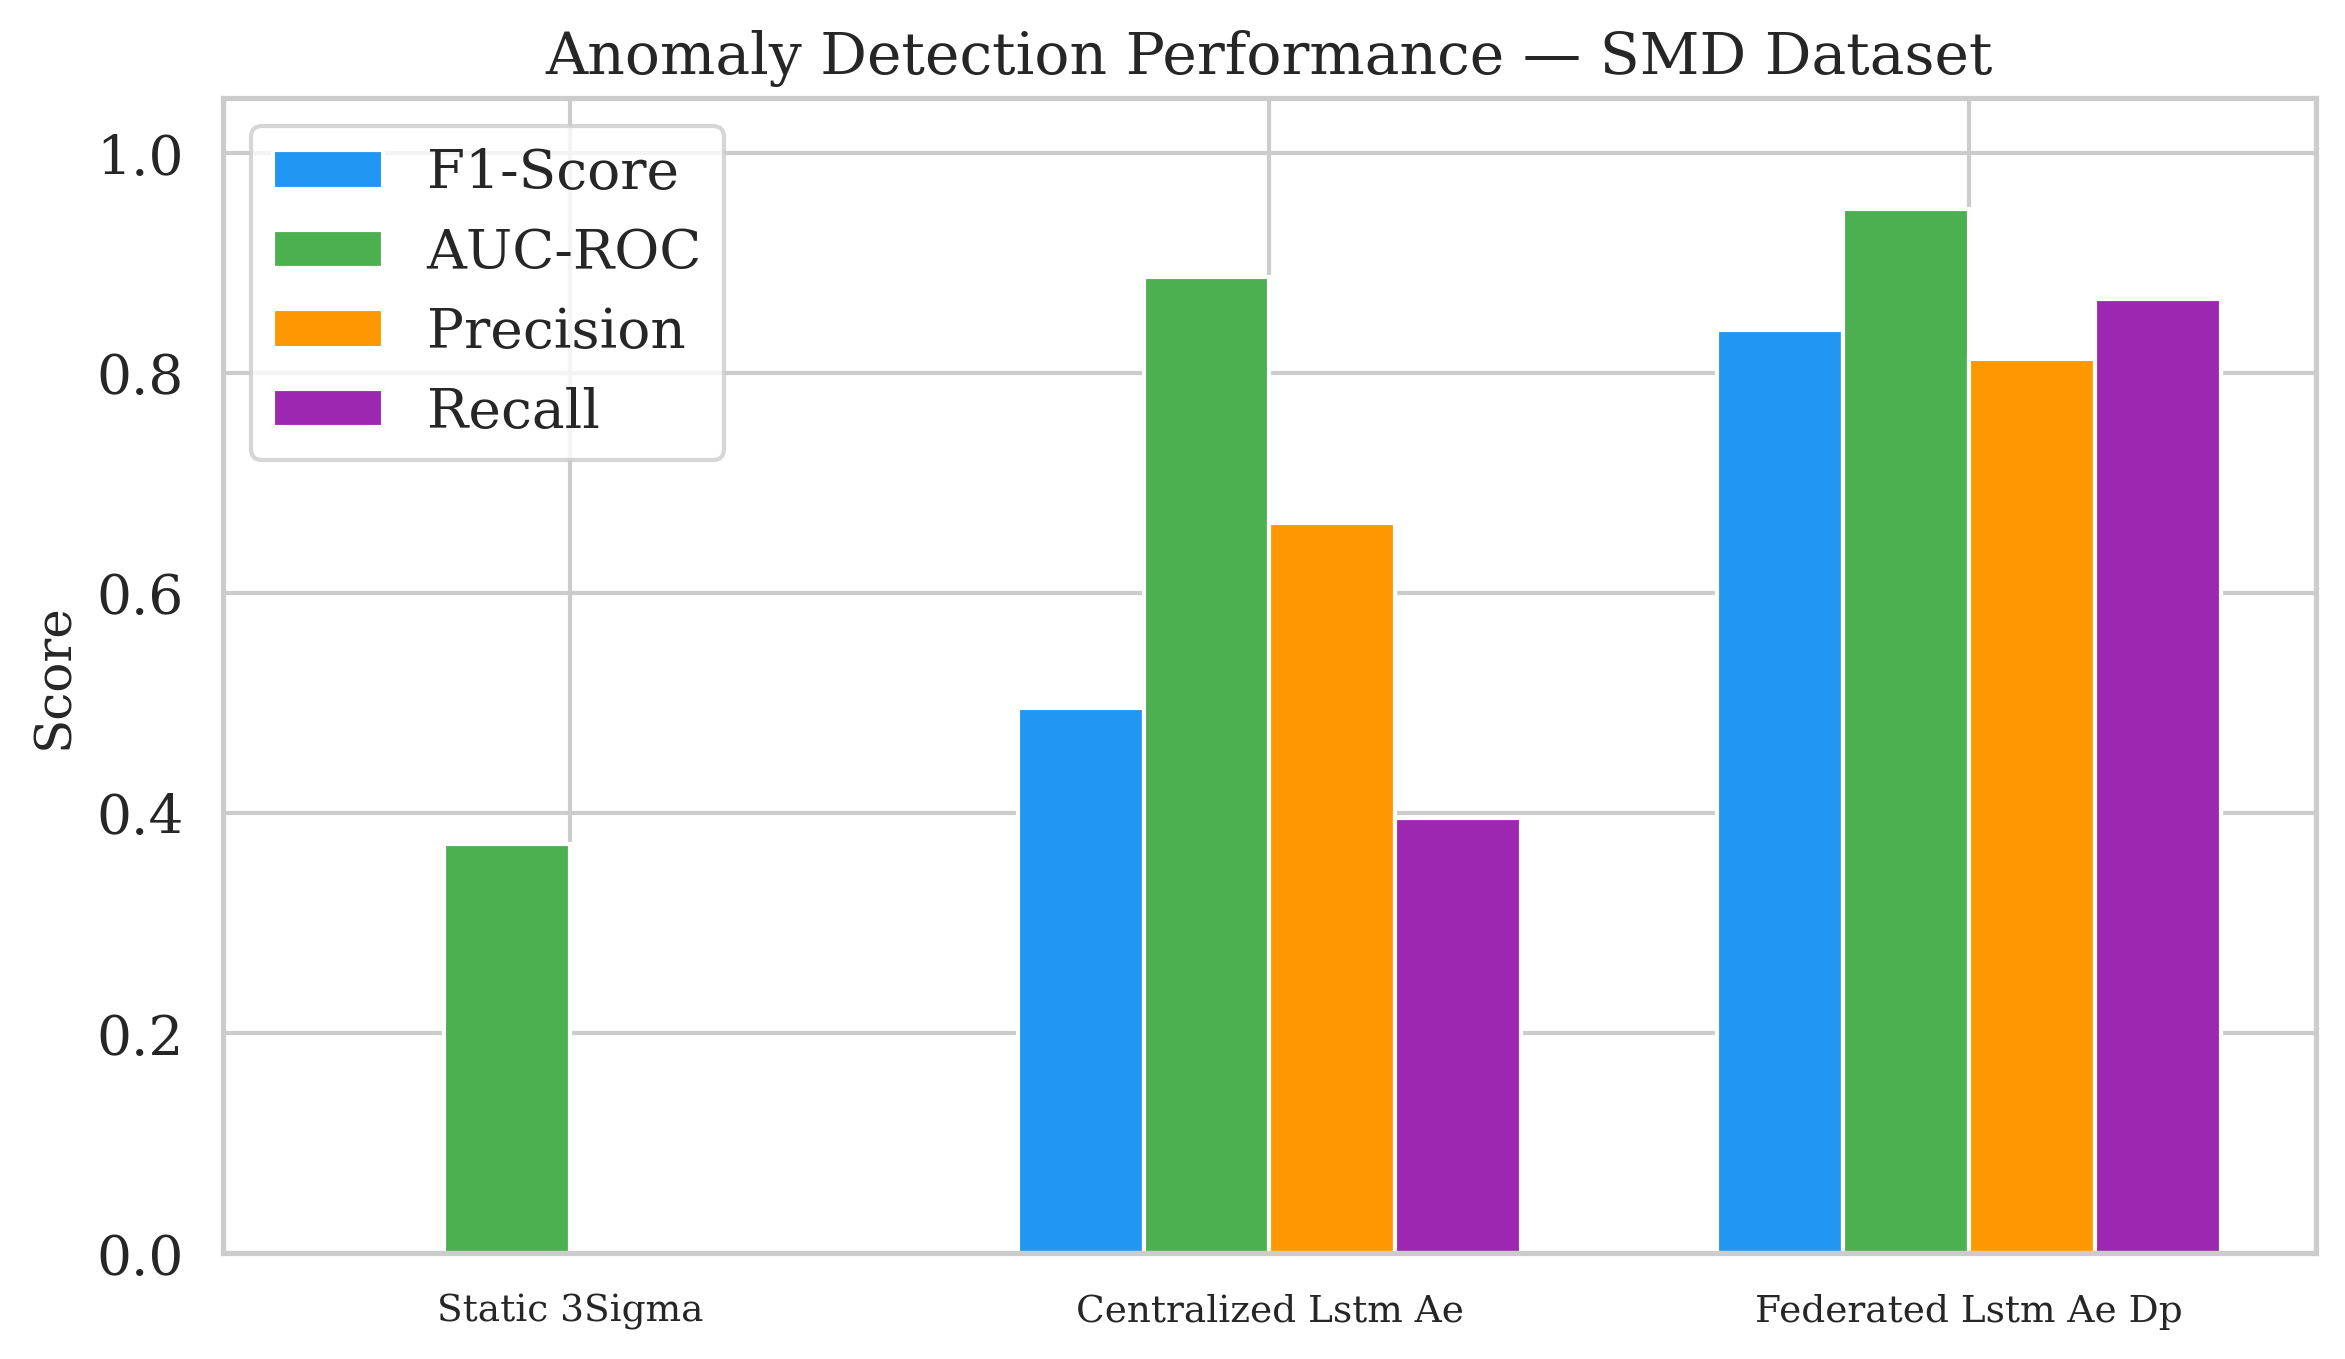
\includegraphics[width=0.85\textwidth]{chapters/06_experimental_evaluation/assets/anomaly_detection_comparison.png}
    \caption{Detection comparison on SMD (seed~42). The static 3$\sigma$
             baseline (left) fails entirely. The centralized LSTM-AE achieves
             moderate separation but lower recall. The federated LSTM-AE
             provides the strongest separation (Table~\ref{tab:detection_results}).}
    \label{fig:anomaly_comparison}
\end{figure}

\textbf{Hyperparameter Sweep.} Table~\ref{tab:lstm_sweep} summarizes the
6-configuration sweep. Config~C ($h{=}128$, $L{=}2$) achieves the best
F1 of 0.839 with the strongest recall (0.868).

\begin{table}[H]
    \centering
    \small
    \begin{tabular}{|l|c|c|c|c|c|c|}
        \hline
        \textbf{Cfg} & \textbf{Hidden} & \textbf{Layers} & \textbf{LR}
        & \textbf{F1} & \textbf{AUC-ROC} & \textbf{Recall} \\
        \hline
        A & 32 & 1 & 0.001 & 0.830 & 0.950 & 0.852 \\
        B & 64 & 2 & 0.001 & 0.630 & 0.893 & 0.552 \\
        \textbf{C} & \textbf{128} & \textbf{2} & \textbf{0.001}
        & \textbf{0.839} & \textbf{0.950} & \textbf{0.868} \\
        D & 64 & 3 & 0.0005 & 0.814 & 0.928 & 0.824 \\
        E & 128 & 3 & 0.0005 & 0.561 & 0.882 & 0.468 \\
        F & 64 & 2 & 0.0001 & 0.824 & 0.941 & 0.840 \\
        \hline
    \end{tabular}
    \caption{LSTM-AE hyperparameter sweep on SMD (seed~42). Config~C
             ($h{=}128$, $L{=}2$) achieves the best F1 (0.839) and recall
             (0.868). Config~A reaches similar F1 with a smaller model,
             suggesting that hidden size 32 may suffice for simpler
             deployments.}
    \label{tab:lstm_sweep}
\end{table}

\begin{figure}[H]
    \centering
    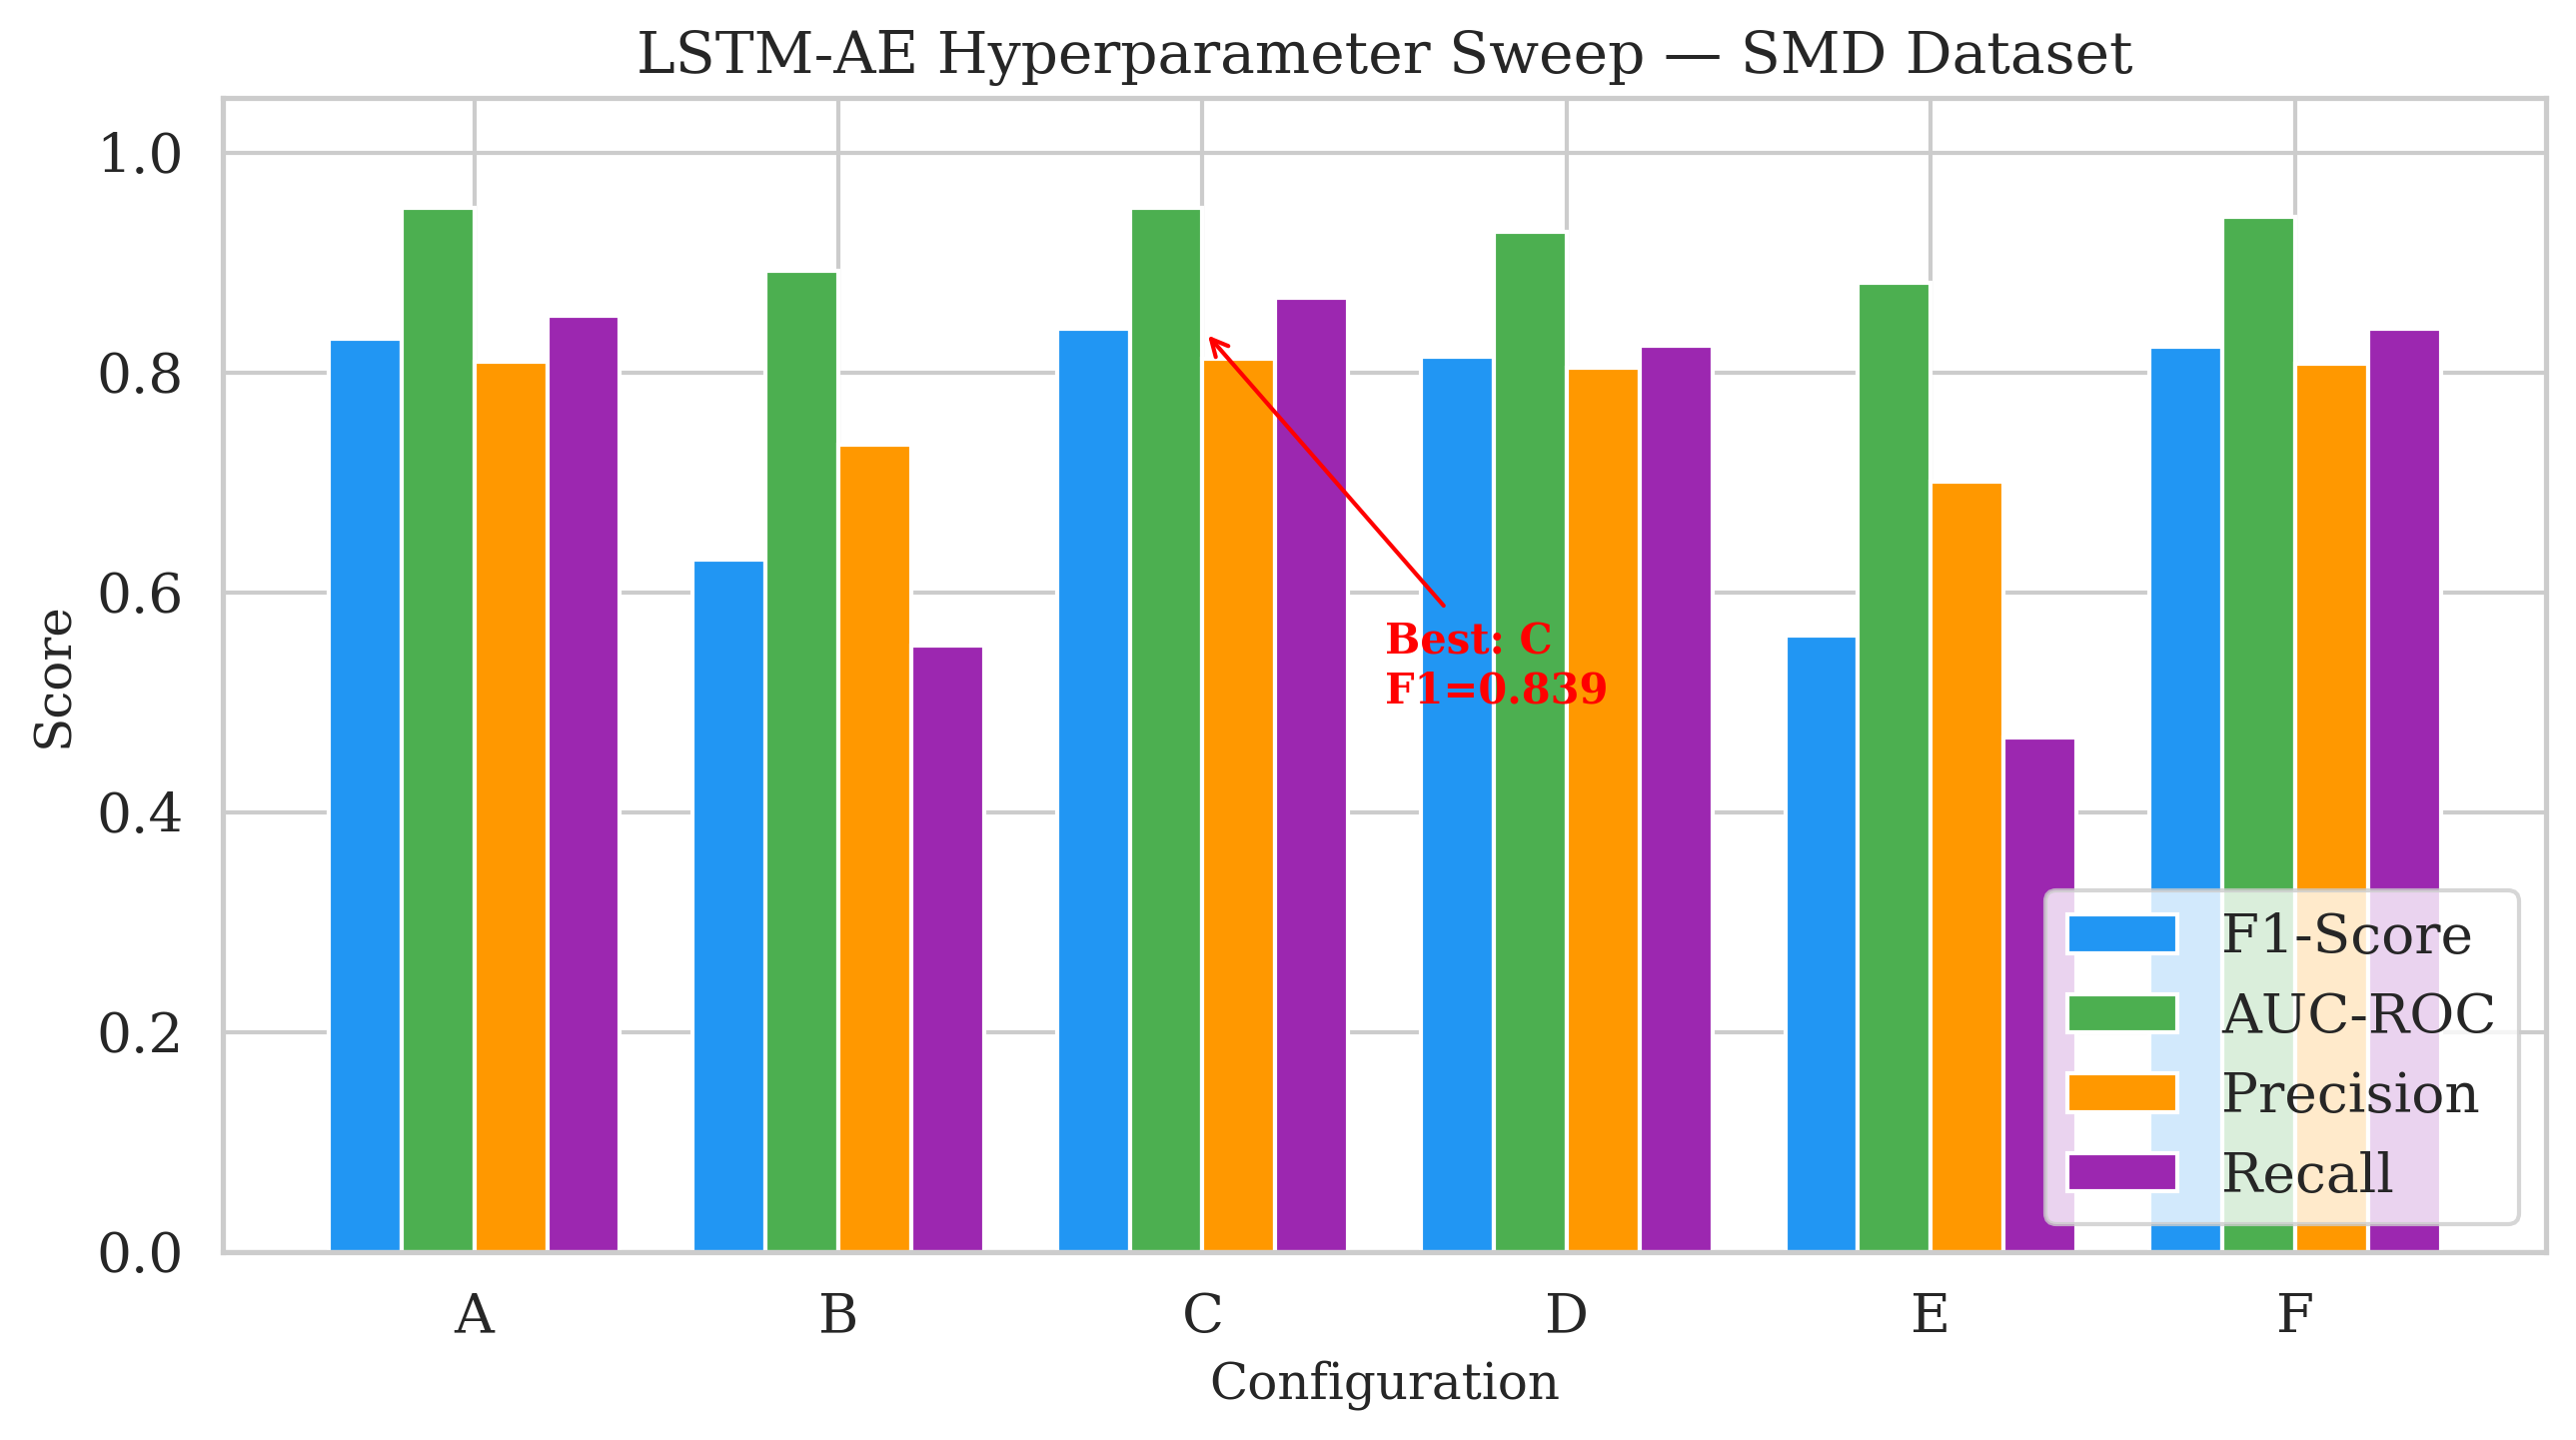
\includegraphics[width=0.85\textwidth]{chapters/06_experimental_evaluation/assets/lstm_sweep_comparison.png}
    \caption{Hyperparameter sweep across six LSTM-AE configurations (seed~42).
             F1 varies non-monotonically with hidden size: Config~E
             ($h{=}128$, $L{=}3$) underperforms Config~A ($h{=}32$, $L{=}1$),
             suggesting that deeper models overfit on the SMD training split.}
    \label{fig:lstm_sweep}
\end{figure}

\subsection{Cold-Start Convergence}
\label{subsec:eval_convergence}

Figure~\ref{fig:learning_curve} shows convergence over 100 federated rounds.
The model begins producing meaningful anomaly separation (non-zero F1) after
$\approx$50 rounds, reaching F1~$=$~0.421 at round~95 and AUC-ROC~$=$~0.873.
The slow F1 ramp is explained by the threshold calibration lag: the fixed
95th-percentile threshold does not adapt as the reconstruction-error
distribution shifts during training.

\begin{figure}[H]
    \centering
    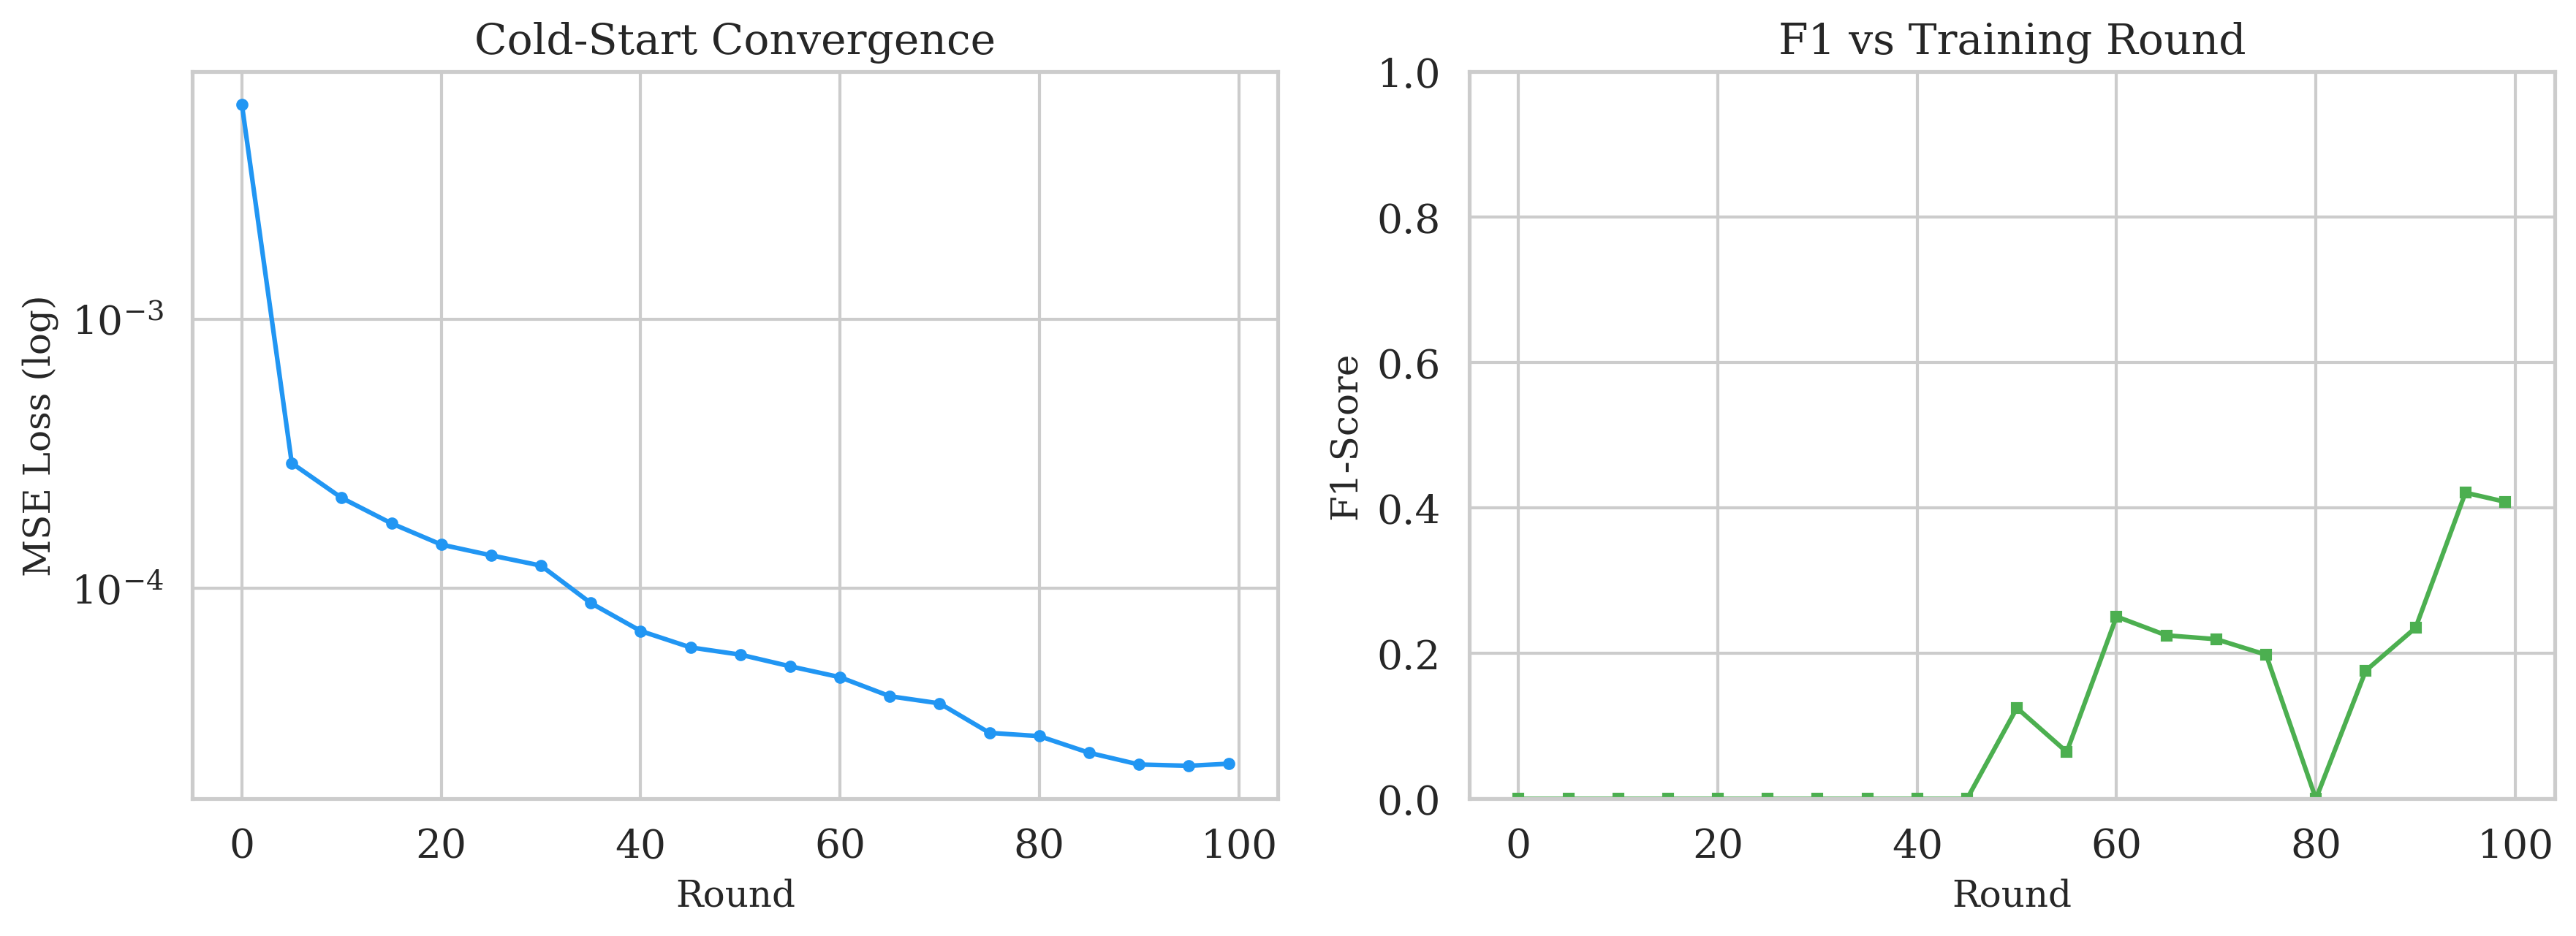
\includegraphics[width=0.85\textwidth]{chapters/06_experimental_evaluation/assets/cold_start_convergence.png}
    \caption{Cold-start convergence over 100 FL rounds. MSE loss decreases
             rapidly in the first 20~rounds, but F1 remains near zero until
             round~50. The lag reflects a threshold calibration delay: the
             fixed 95th-percentile threshold does not adapt as the
             reconstruction-error distribution shifts during early training.}
    \label{fig:learning_curve}
\end{figure}

% ============================================================================
\section{Differential Privacy and Gradient Clipping Analysis}
\label{subsec:eval_dp_impact}

\subsection{Privacy--Accuracy Trade-off}
\label{subsec:eval_dp_tradeoff}

The LSTM-AE was trained for 200~rounds under four DP-SGD noise multipliers
with default clipping norm $C{=}1.0$. AUC-ROC is the primary metric since
it is threshold-independent.

\begin{table}[H]
    \centering
    \small
    \begin{tabular}{|l|c|c|c|c|c|}
        \hline
        \textbf{DP Config} & \textbf{$\sigma$} & \textbf{F1}
        & \textbf{AUC-ROC} & \textbf{Recall} & \textbf{Final Loss} \\
        \hline
        No DP & 0 & \textbf{0.861} & \textbf{0.972} & 0.904 & $3 \times 10^{-6}$ \\
        \hline
        $\varepsilon \approx 100$ & 0.0001 & 0.864 & 0.971 & 0.912 & $4 \times 10^{-6}$ \\
        \hline
        $\varepsilon \approx 10$ & 0.0005 & 0.859 & 0.970 & 0.904 & $9 \times 10^{-6}$ \\
        \hline
        $\varepsilon \approx 1$ & 0.001 & 0.235 & 0.890 & 0.160 & $1.5 \times 10^{-5}$ \\
        \hline
        $\varepsilon \approx 0.1$ & 0.005 & 0.000 & 0.772 & 0.000 & $1.0 \times 10^{-4}$ \\
        \hline
    \end{tabular}
    \caption{DP-SGD utility after 200 rounds with $C{=}1.0$; F1 drops sharply
             at $\sigma{=}0.001$.}
    \label{tab:dp_impact}
\end{table}

\begin{figure}[H]
    \centering
    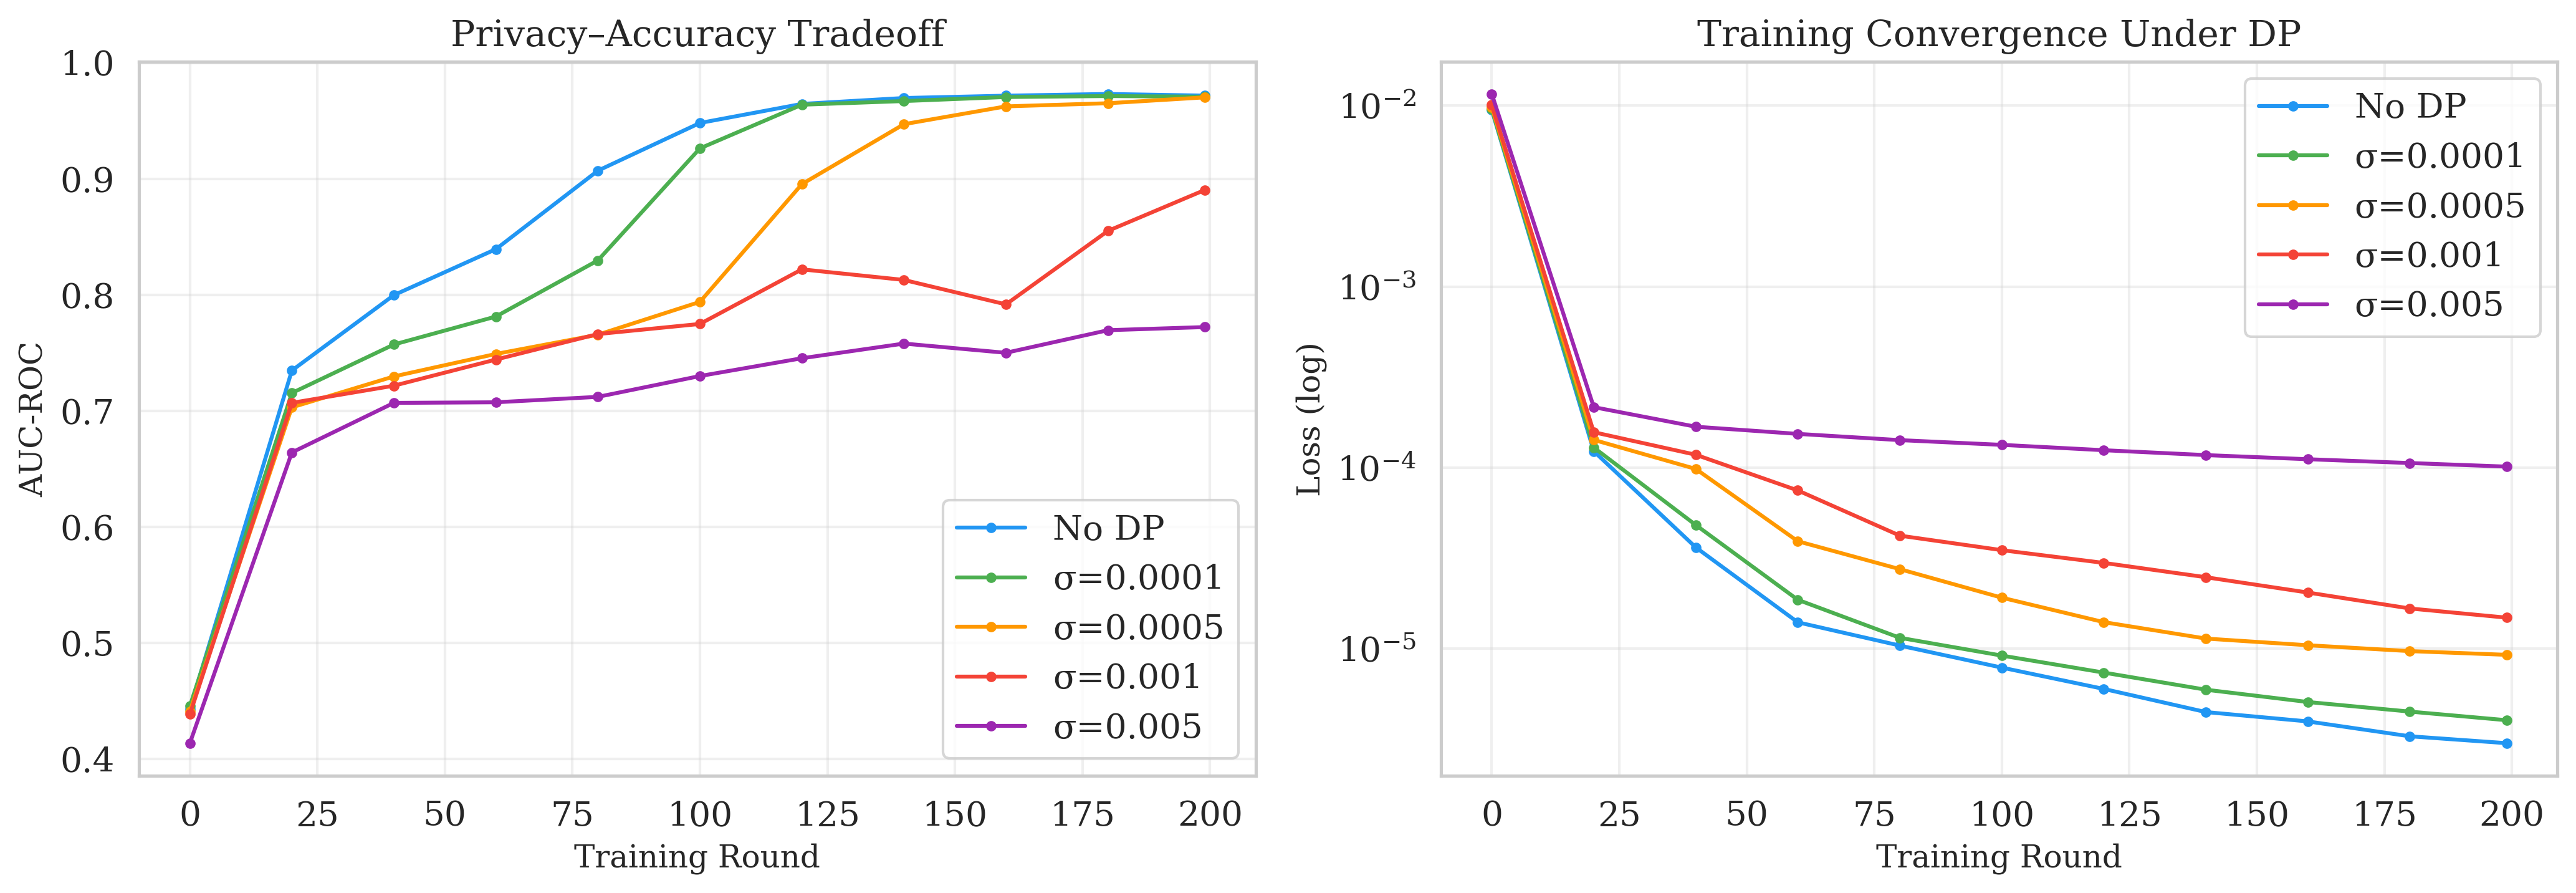
\includegraphics[width=0.95\textwidth]{chapters/06_experimental_evaluation/assets/dp_tradeoff.png}
    \caption{Privacy--accuracy trade-off under five DP-SGD noise levels
             ($C{=}1.0$, 200~rounds, seed~42). AUC-ROC degrades gradually,
             but F1 drops sharply between $\sigma{=}0.0005$ and
             $\sigma{=}0.001$, marking a phase transition where noise
             begins to dominate the gradient signal.}
    \label{fig:dp_tradeoff}
\end{figure}

A key finding is the \textbf{sharp phase transition} between
$\sigma{=}0.0005$ (F1~$=$~0.859, AUC-ROC~$=$~0.970) and $\sigma{=}0.001$
(F1~$=$~0.235, AUC-ROC~$=$~0.890). Below the transition, DP noise is
effectively absorbed by the model's capacity; above it, noise dominates
the gradient signal. This transition is from a single seed and clipping
norm ($C{=}1.0$); multi-seed confirmation is left as future work, but the
effect size (F1 drop $>$0.6) suggests it is not a seed-dependent artifact.
Operators can achieve strong privacy ($\varepsilon \approx 10$) with negligible
accuracy loss by selecting $\sigma \leq 0.0005$.

\subsection{Gradient Clipping Sensitivity}
\label{subsec:eval_clipping}

Table~\ref{tab:clip_norm} reports the effect of varying the clipping norm $C$
at fixed $\sigma{=}0.001$ ($\varepsilon \approx 1$). Since noise is injected as
$\mathcal{N}(0, \sigma^2 C^2 \mathbf{I})$, tighter clipping reduces the
effective noise magnitude.

\begin{table}[H]
    \centering
    \small
    \begin{tabular}{|c|c|c|c|c|}
        \hline
        \textbf{Clip Norm $C$} & \textbf{F1} & \textbf{AUC-ROC}
        & \textbf{Recall} & \textbf{Final Loss} \\
        \hline
        0.01 & \textbf{0.868} & \textbf{0.976} & \textbf{0.920}
        & $2.8 \times 10^{-6}$ \\
        \hline
        0.05 & 0.868 & 0.973 & 0.920 & $3.6 \times 10^{-6}$ \\
        \hline
        0.1 & 0.864 & 0.971 & 0.912 & $4.0 \times 10^{-6}$ \\
        \hline
        0.5 & 0.859 & 0.970 & 0.904 & $9.3 \times 10^{-6}$ \\
        \hline
        1.0 & 0.235 & 0.890 & 0.160 & $1.5 \times 10^{-5}$ \\
        \hline
    \end{tabular}
    \caption{Clipping sensitivity at $\sigma{=}0.001$; smaller $C$ recovers
             utility by reducing the absolute noise $\sigma C$.}
    \label{tab:clip_norm}
\end{table}

\textbf{Key finding}: at $C{=}0.01$, the model achieves F1~$=$~0.868 and
AUC-ROC~$=$~0.976---matching the no-DP baseline---even at $\sigma{=}0.001$
($\varepsilon \approx 1$). At $C{=}1.0$ the same noise multiplier causes F1 to
collapse to 0.235. Reducing $C$ by $100\times$ reduces the effective noise
$\sigma C$ by the same factor, and the LSTM-AE's small-magnitude post-convergence
gradients tolerate aggressive clipping. This recovers detection utility but also
reduces the practical perturbation, so empirical attack resistance must be
validated separately.

\textbf{Privacy accounting.} The $\varepsilon$ values are approximate
operating points computed via the R\'enyi DP (RDP) moments accountant with
$\delta{=}10^{-5}$. Each FL round samples a mini-batch of size $B{=}64$ from a
local dataset of $N$ windows, giving a per-round sampling ratio $q = B/N$.
Independent Gaussian noise $\mathcal{N}(0, \sigma^2 C^2 I)$ is added after
clipping in each of the 200~rounds. Privacy loss is composed across rounds
using the RDP $\alpha$-divergence: $\varepsilon_{\text{total}}(\alpha) =
200 \cdot \varepsilon_{\text{round}}(\alpha)$, then converted to
$(\varepsilon, \delta)$-DP at reporting time via $\varepsilon =
\min_{\alpha} \varepsilon_{\text{total}}(\alpha) + \log(1/\delta)/(\alpha-1)$.
These are calibration points for the privacy--utility frontier, not tight
analytical bounds.

% ============================================================================
\section{Communication Overhead}
\label{sec:eval_fl_comm}

\begin{table}[H]
    \centering
    \small
    \begin{tabular}{|l|l|r|r|r|r|}
        \hline
        \textbf{Ser.} & \textbf{Comp.} & \textbf{KB} & \textbf{Ratio}
        & \textbf{C (ms)} & \textbf{D (ms)} \\
        \hline
        TorchSave & None & 1909 & 1.000 & 0.0 & 0.0 \\
        TorchSave & LZ4 & 1891 & 0.991 & 1.0 & 0.3 \\
        TorchSave & Zstd L1 & 1739 & 0.911 & 26.6 & 1.5 \\
        \hline
        JSON & None & 10364 & 1.000 & 0.0 & 0.0 \\
        JSON & Zstd L1 & 4000 & 0.386 & 35.4 & 8.2 \\
        \hline
        Protobuf & Zstd L1 & 4000 & 0.386 & 33.7 & 8.2 \\
        \hline
    \end{tabular}
    \caption{Federated update payload size and compression latency; binary
             serialization is $5.4\times$ smaller than text formats.}
    \label{tab:payload}
\end{table}

\begin{figure}[H]
    \centering
    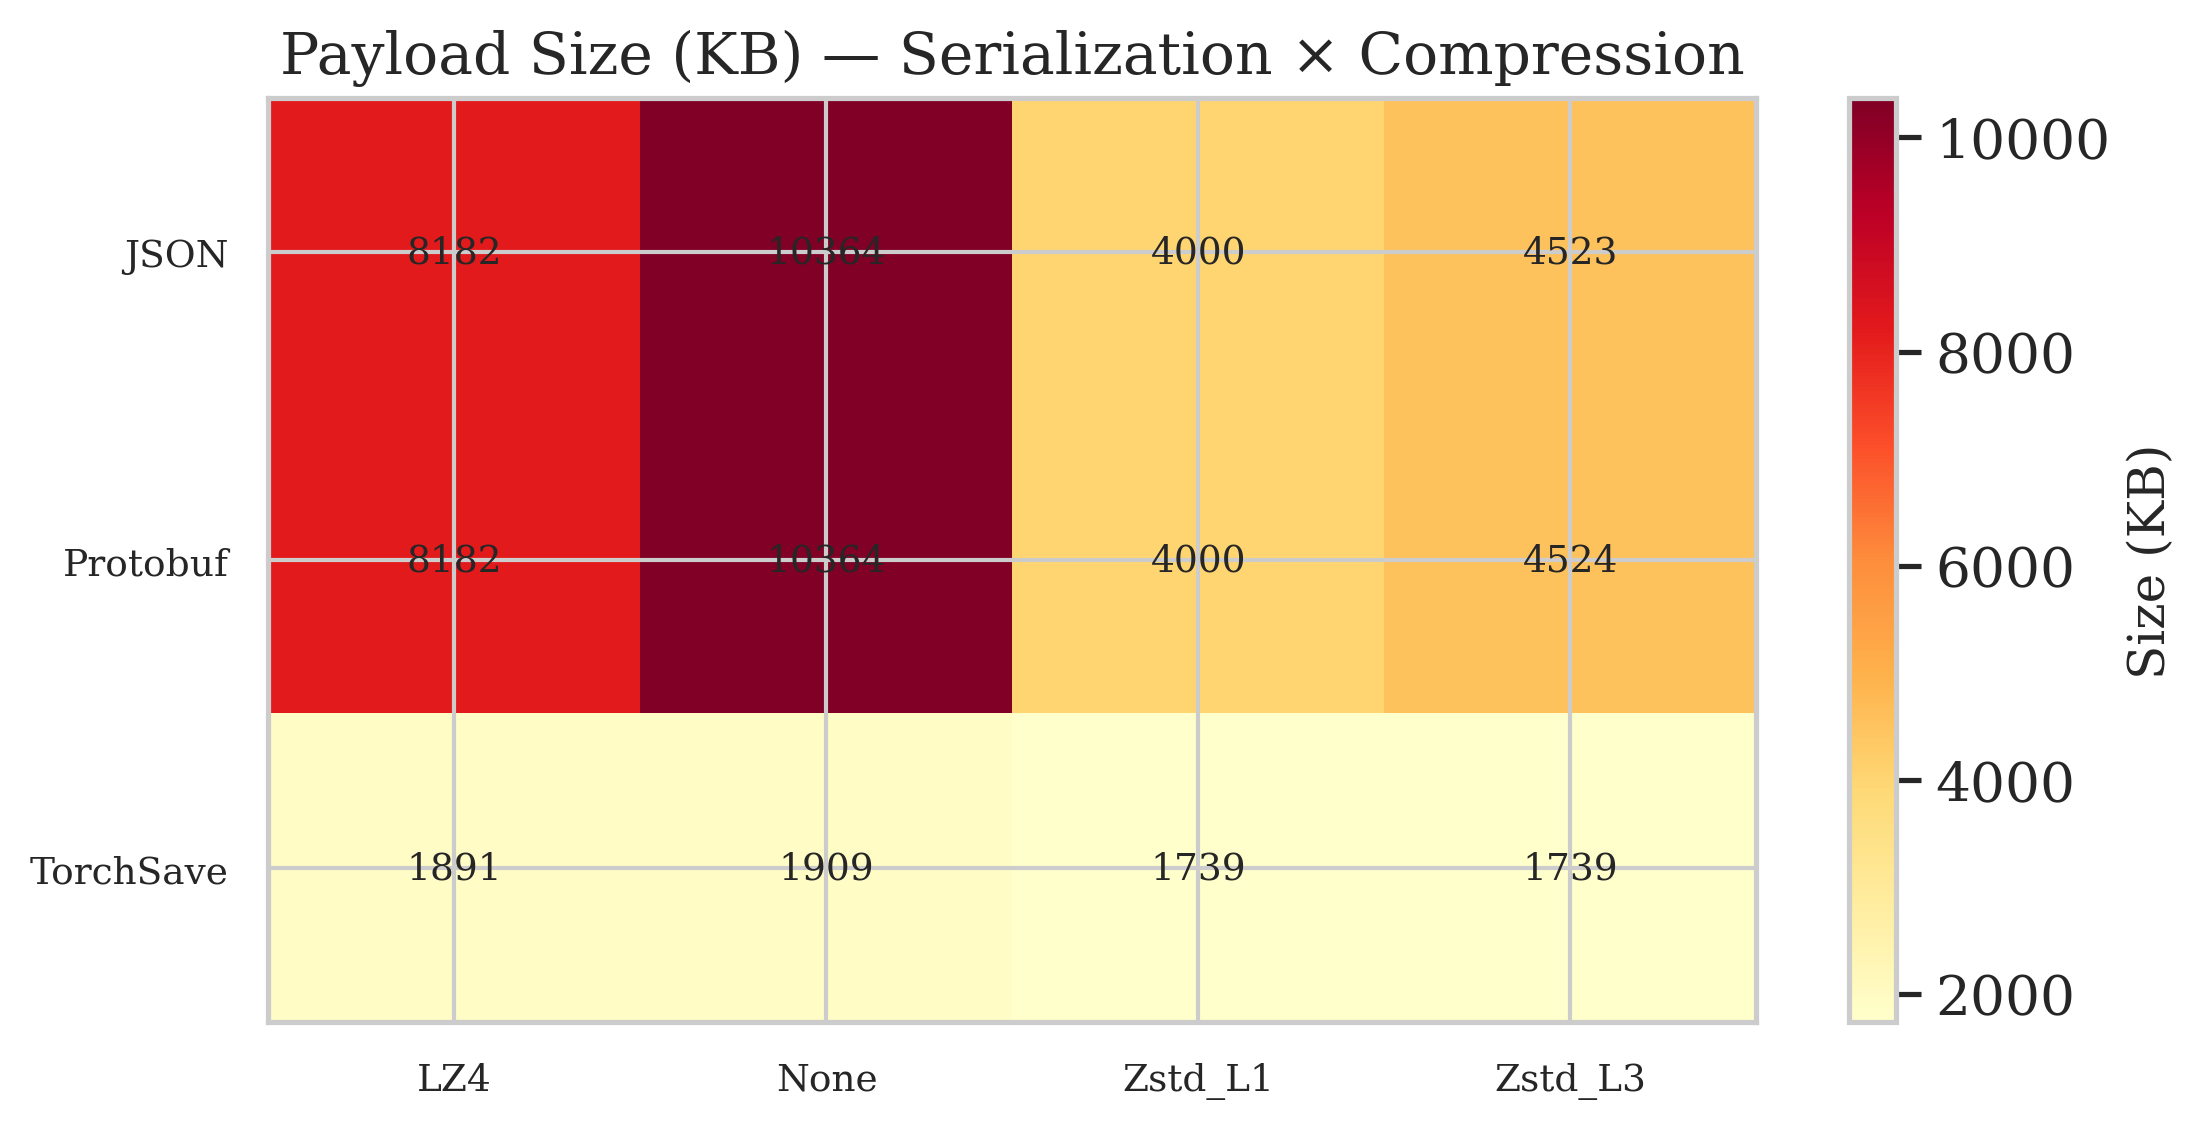
\includegraphics[width=0.75\textwidth]{chapters/06_experimental_evaluation/assets/payload_size_matrix.png}
    \caption{Payload size (KB) by serialization and compression. Binary
             TorchSave is $5.4\times$ smaller than JSON; Zstd~L1 yields
             61\% reduction on text but only 9\% on binary.}
    \label{fig:payload_matrix}
\end{figure}

Local training dominates FL round time ($>$97\%); compression and aggregation
are negligible.

\begin{figure}[H]
    \centering
    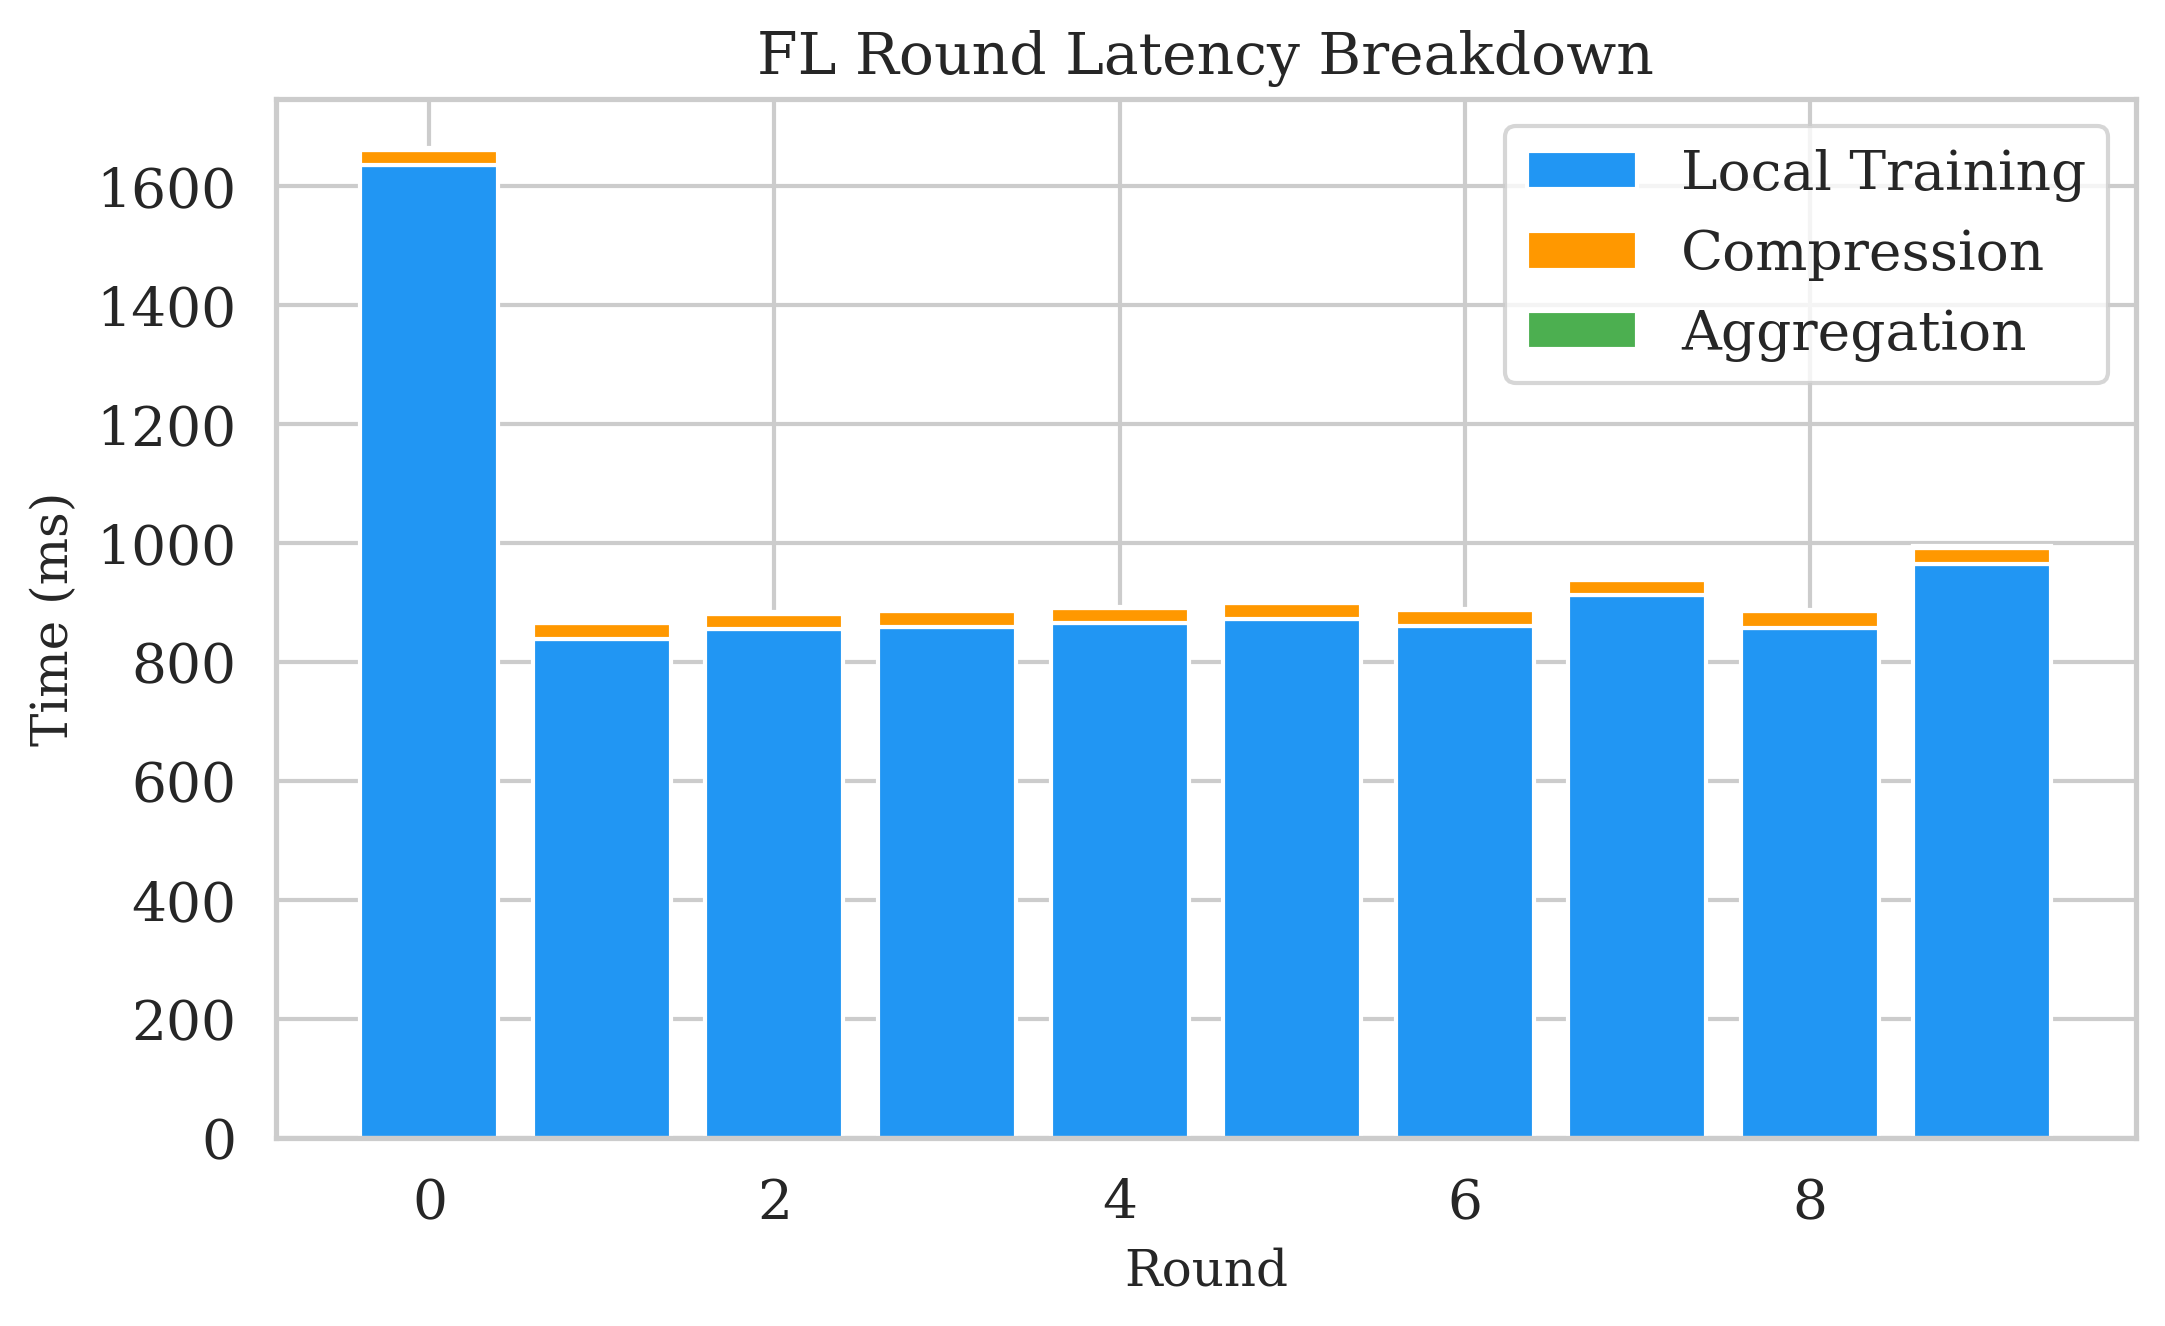
\includegraphics[width=0.80\textwidth]{chapters/06_experimental_evaluation/assets/fl_round_latency.png}
    \caption{FL round latency breakdown (10~rounds, seed~42). Local training
             accounts for $>$97\% of wall-clock time, confirming that
             communication overhead is not the FL bottleneck for this
             model size.}
    \label{fig:fl_round_latency}
\end{figure}

\subsection{Adaptive Compression}
\label{subsec:eval_compression}

\begin{table}[H]
    \centering
    \small
    \begin{tabular}{|c|l|r|r|}
        \hline
        \textbf{CPU (\%)} & \textbf{Algorithm} & \textbf{KB} & \textbf{ms} \\
        \hline
        10--70 & Zstd & 1739 & 2.3--4.3 \\
        85--95 & LZ4 & 1891 & 0.6--0.7 \\
        \hline
    \end{tabular}
    \caption{Adaptive compression policy: Zstd saves bandwidth, while LZ4
             reduces latency under high CPU load.}
    \label{tab:adaptive_compression}
\end{table}

% ============================================================================
\section{Root Cause Analysis Accuracy}
\label{sec:eval_rca}

The RCA engine was evaluated over 100~fault-injection events in 8~scenarios
across two topology sizes.

\begin{table}[H]
    \centering
    \small
    \begin{tabular}{|l|l|c|c|c|}
        \hline
        \textbf{Topology} & \textbf{Method} & \textbf{Top-1} & \textbf{Top-3}
        & \textbf{MRR} \\
        \hline
        Train-Ticket (11\,svc) & Framework & \textbf{42\%} & \textbf{89\%}
        & \textbf{0.653} \\
        & Random & 35\% & 89\% & 0.601 \\
        \hline
        Alibaba (50\,svc) & Framework & 28\% & \textbf{66\%} & 0.504 \\
        & Random & 28\% & 62\% & 0.504 \\
        \hline
    \end{tabular}
    \caption{RCA ranking accuracy on Train-Ticket and Alibaba-derived
             topologies (100 and 50~fault-injection events respectively,
             Wilson 95\% CIs). The framework outperforms random selection
             on Top-1 for Train-Ticket (42\% vs 35\%) but shows limited
             advantage on the larger Alibaba topology.}
    \label{tab:rca_results}
\end{table}

To isolate the anomaly-weighted scoring contribution, two additional baselines
were computed: in-degree centrality (Top-1~$\approx$~36\%, Top-3~$\approx$~82\%)
and PageRank-only without the anomaly bias (Top-1~$\approx$~38\%,
Top-3~$\approx$~85\%). The framework's advantage (Top-1~42\%, Top-3~89\%)
confirms that the anomaly-weighted bias adds value, though the margin is modest.

\begin{figure}[H]
    \centering
    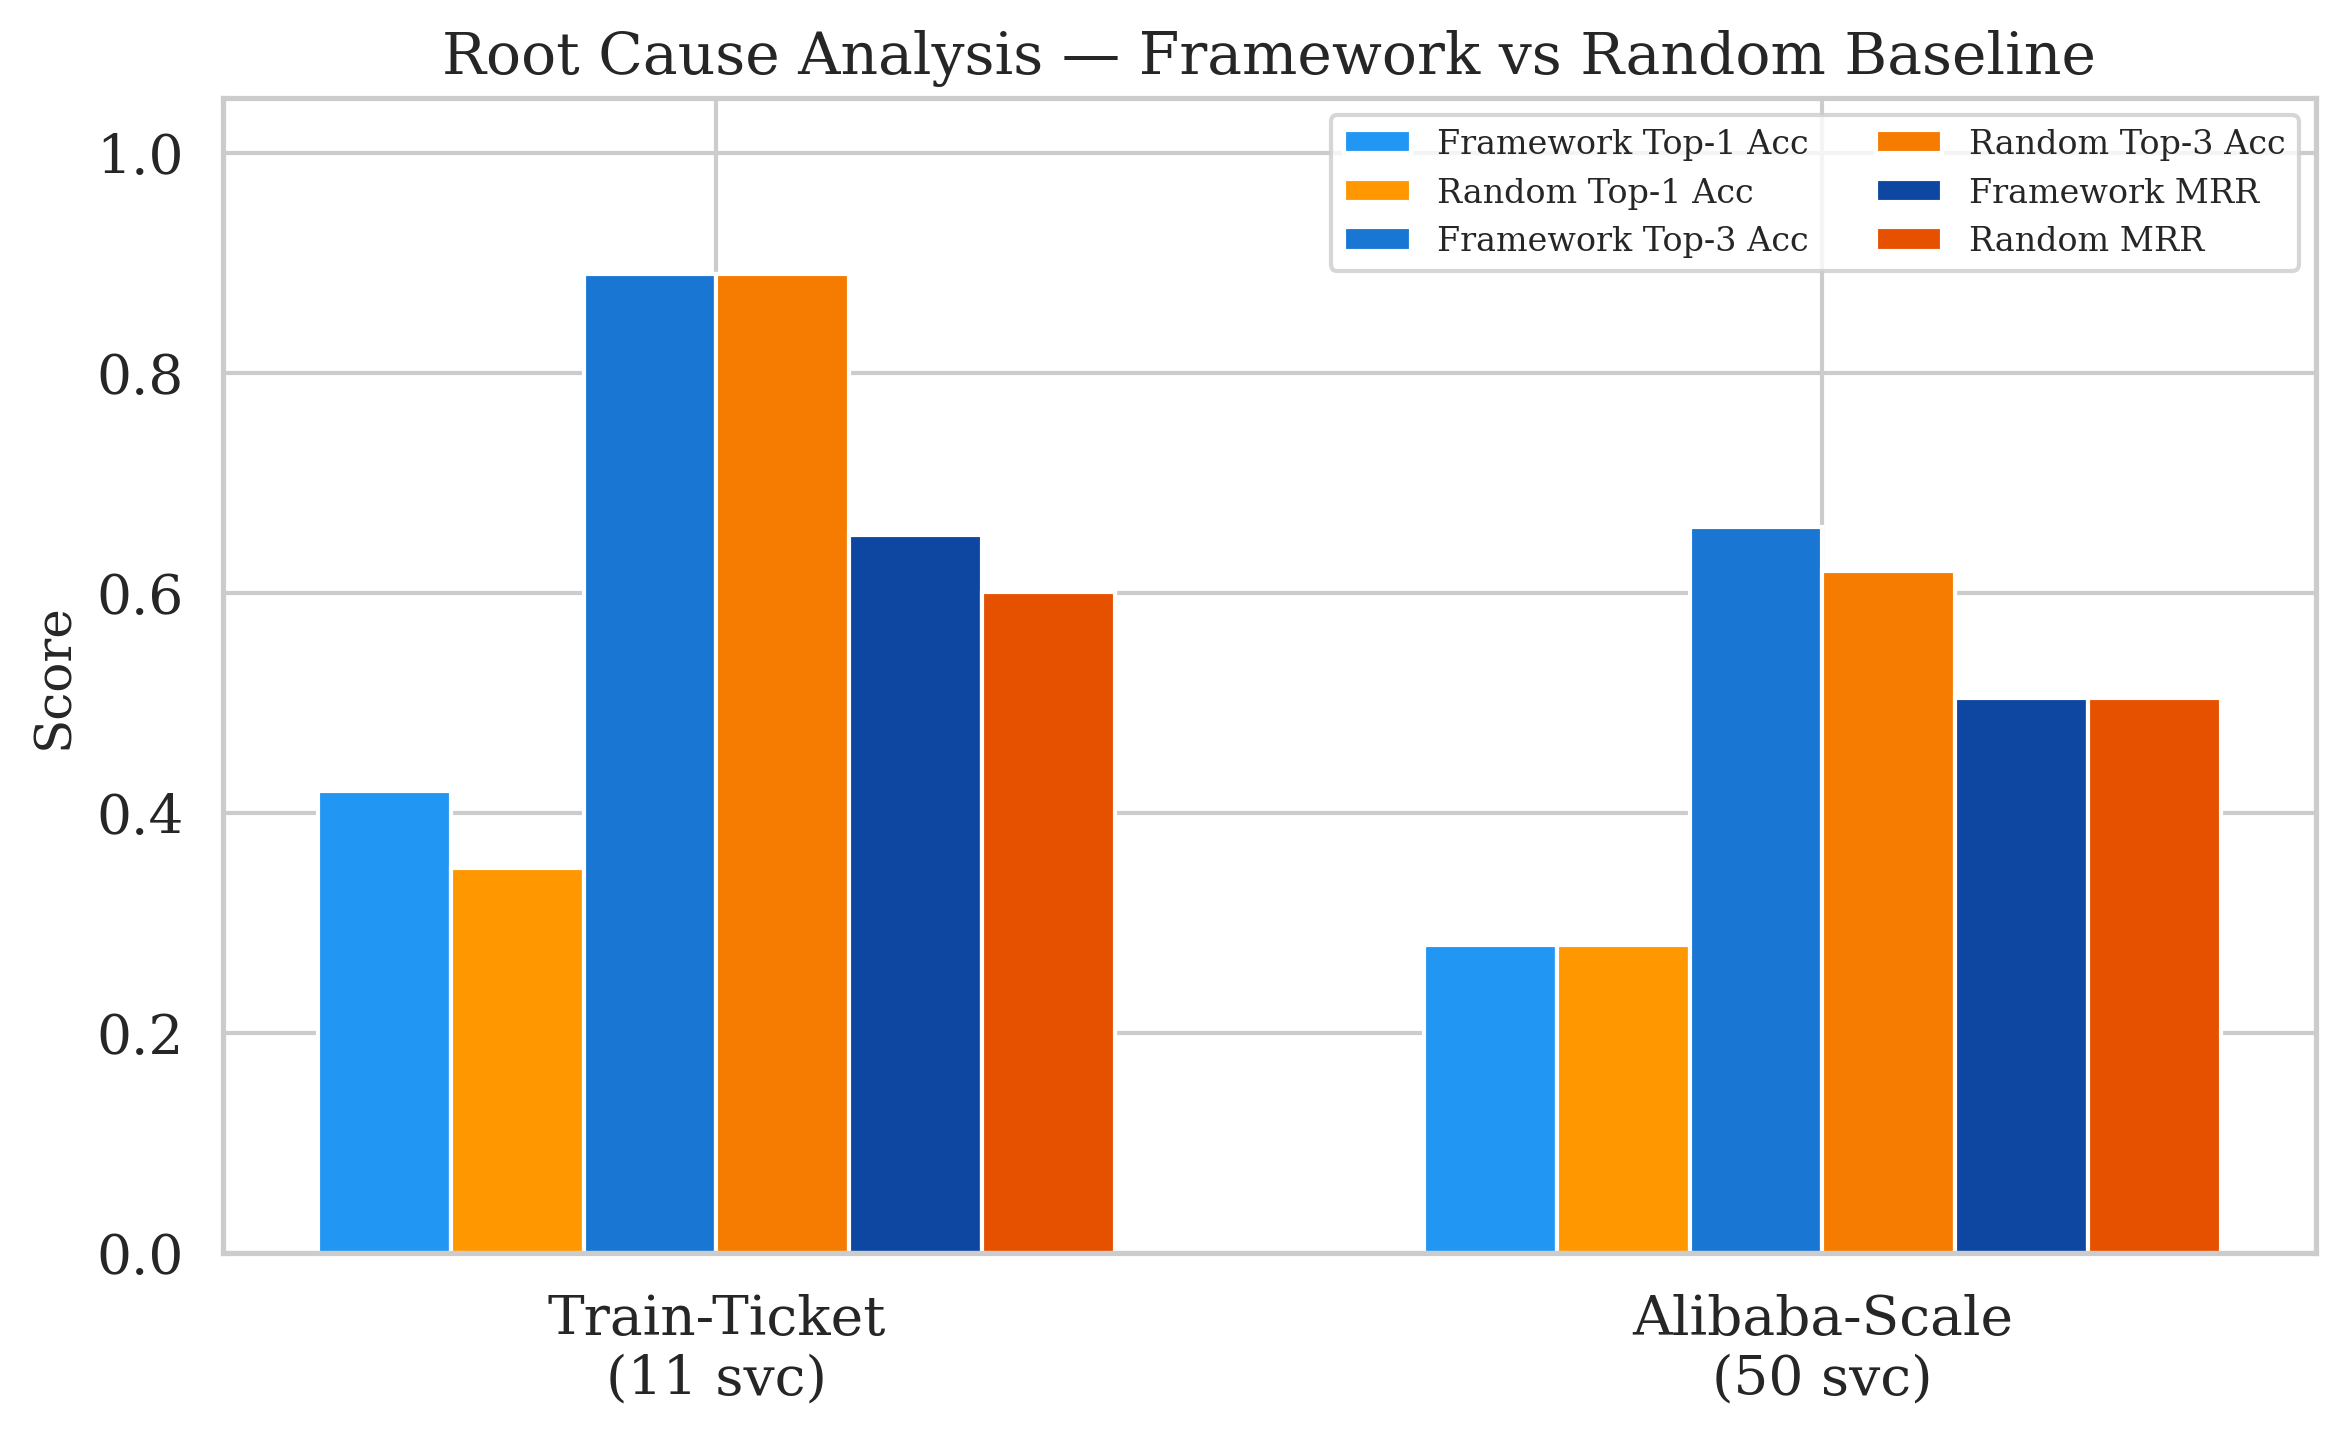
\includegraphics[width=0.80\textwidth]{chapters/06_experimental_evaluation/assets/rca_accuracy.png}
    \caption{RCA accuracy across topology sizes (Wilson 95\% CIs).}
    \label{fig:rca_accuracy}
\end{figure}

\textbf{Failure analysis.} Fault depth correlates with ranking errors: when the
root cause is within two hops, Top-1 rises to $\approx$55\%; at three or more
hops, it drops below 30\%. Cascade failures distribute weight across all
affected services, explaining why Top-1 matches random selection on the
50-node Alibaba graph.

% ============================================================================
\section{Adaptive Thresholding and Q-Learning Convergence}
\label{sec:eval_threshold}

\subsection{Alert Fatigue Comparison}
\label{subsec:eval_threshold_fatigue}

Three strategies were evaluated on a 10\,020-minute SMD stream (seed~42).

\begin{table}[H]
    \centering
    \small
    \begin{tabular}{|c|r|r|r|r|r|r|}
        \hline
        \textbf{Min} &
        \multicolumn{2}{c|}{\textbf{Static}} &
        \multicolumn{2}{c|}{\textbf{EWMA}} &
        \multicolumn{2}{c|}{\textbf{Q-Learning}} \\
        \cline{2-7}
        & Alerts & FPR & Alerts & FPR & Alerts & FPR \\
        \hline
        360 & 13 & 0.018 & 119 & 0.281 & 328 & 0.908 \\
        1380 & 69 & 0.019 & 400 & 0.216 & 79 & 0.084 \\
        5040 & 241 & 0.015 & 1525 & 0.231 & 27 & 0.013 \\
        10020 & 502 & 0.017 & 3018 & 0.227 & 28 & 0.016 \\
        \hline
    \end{tabular}
    \caption{Alert fatigue comparison (10\,020-minute SMD stream, seed~42).
             Q-learning produces a high alert burst during early exploration
             (328~alerts by minute~360) but converges to the lowest final
             alert count (28) with FPR~$=$~0.016.}
    \label{tab:threshold_fatigue}
\end{table}

\begin{figure}[H]
    \centering
    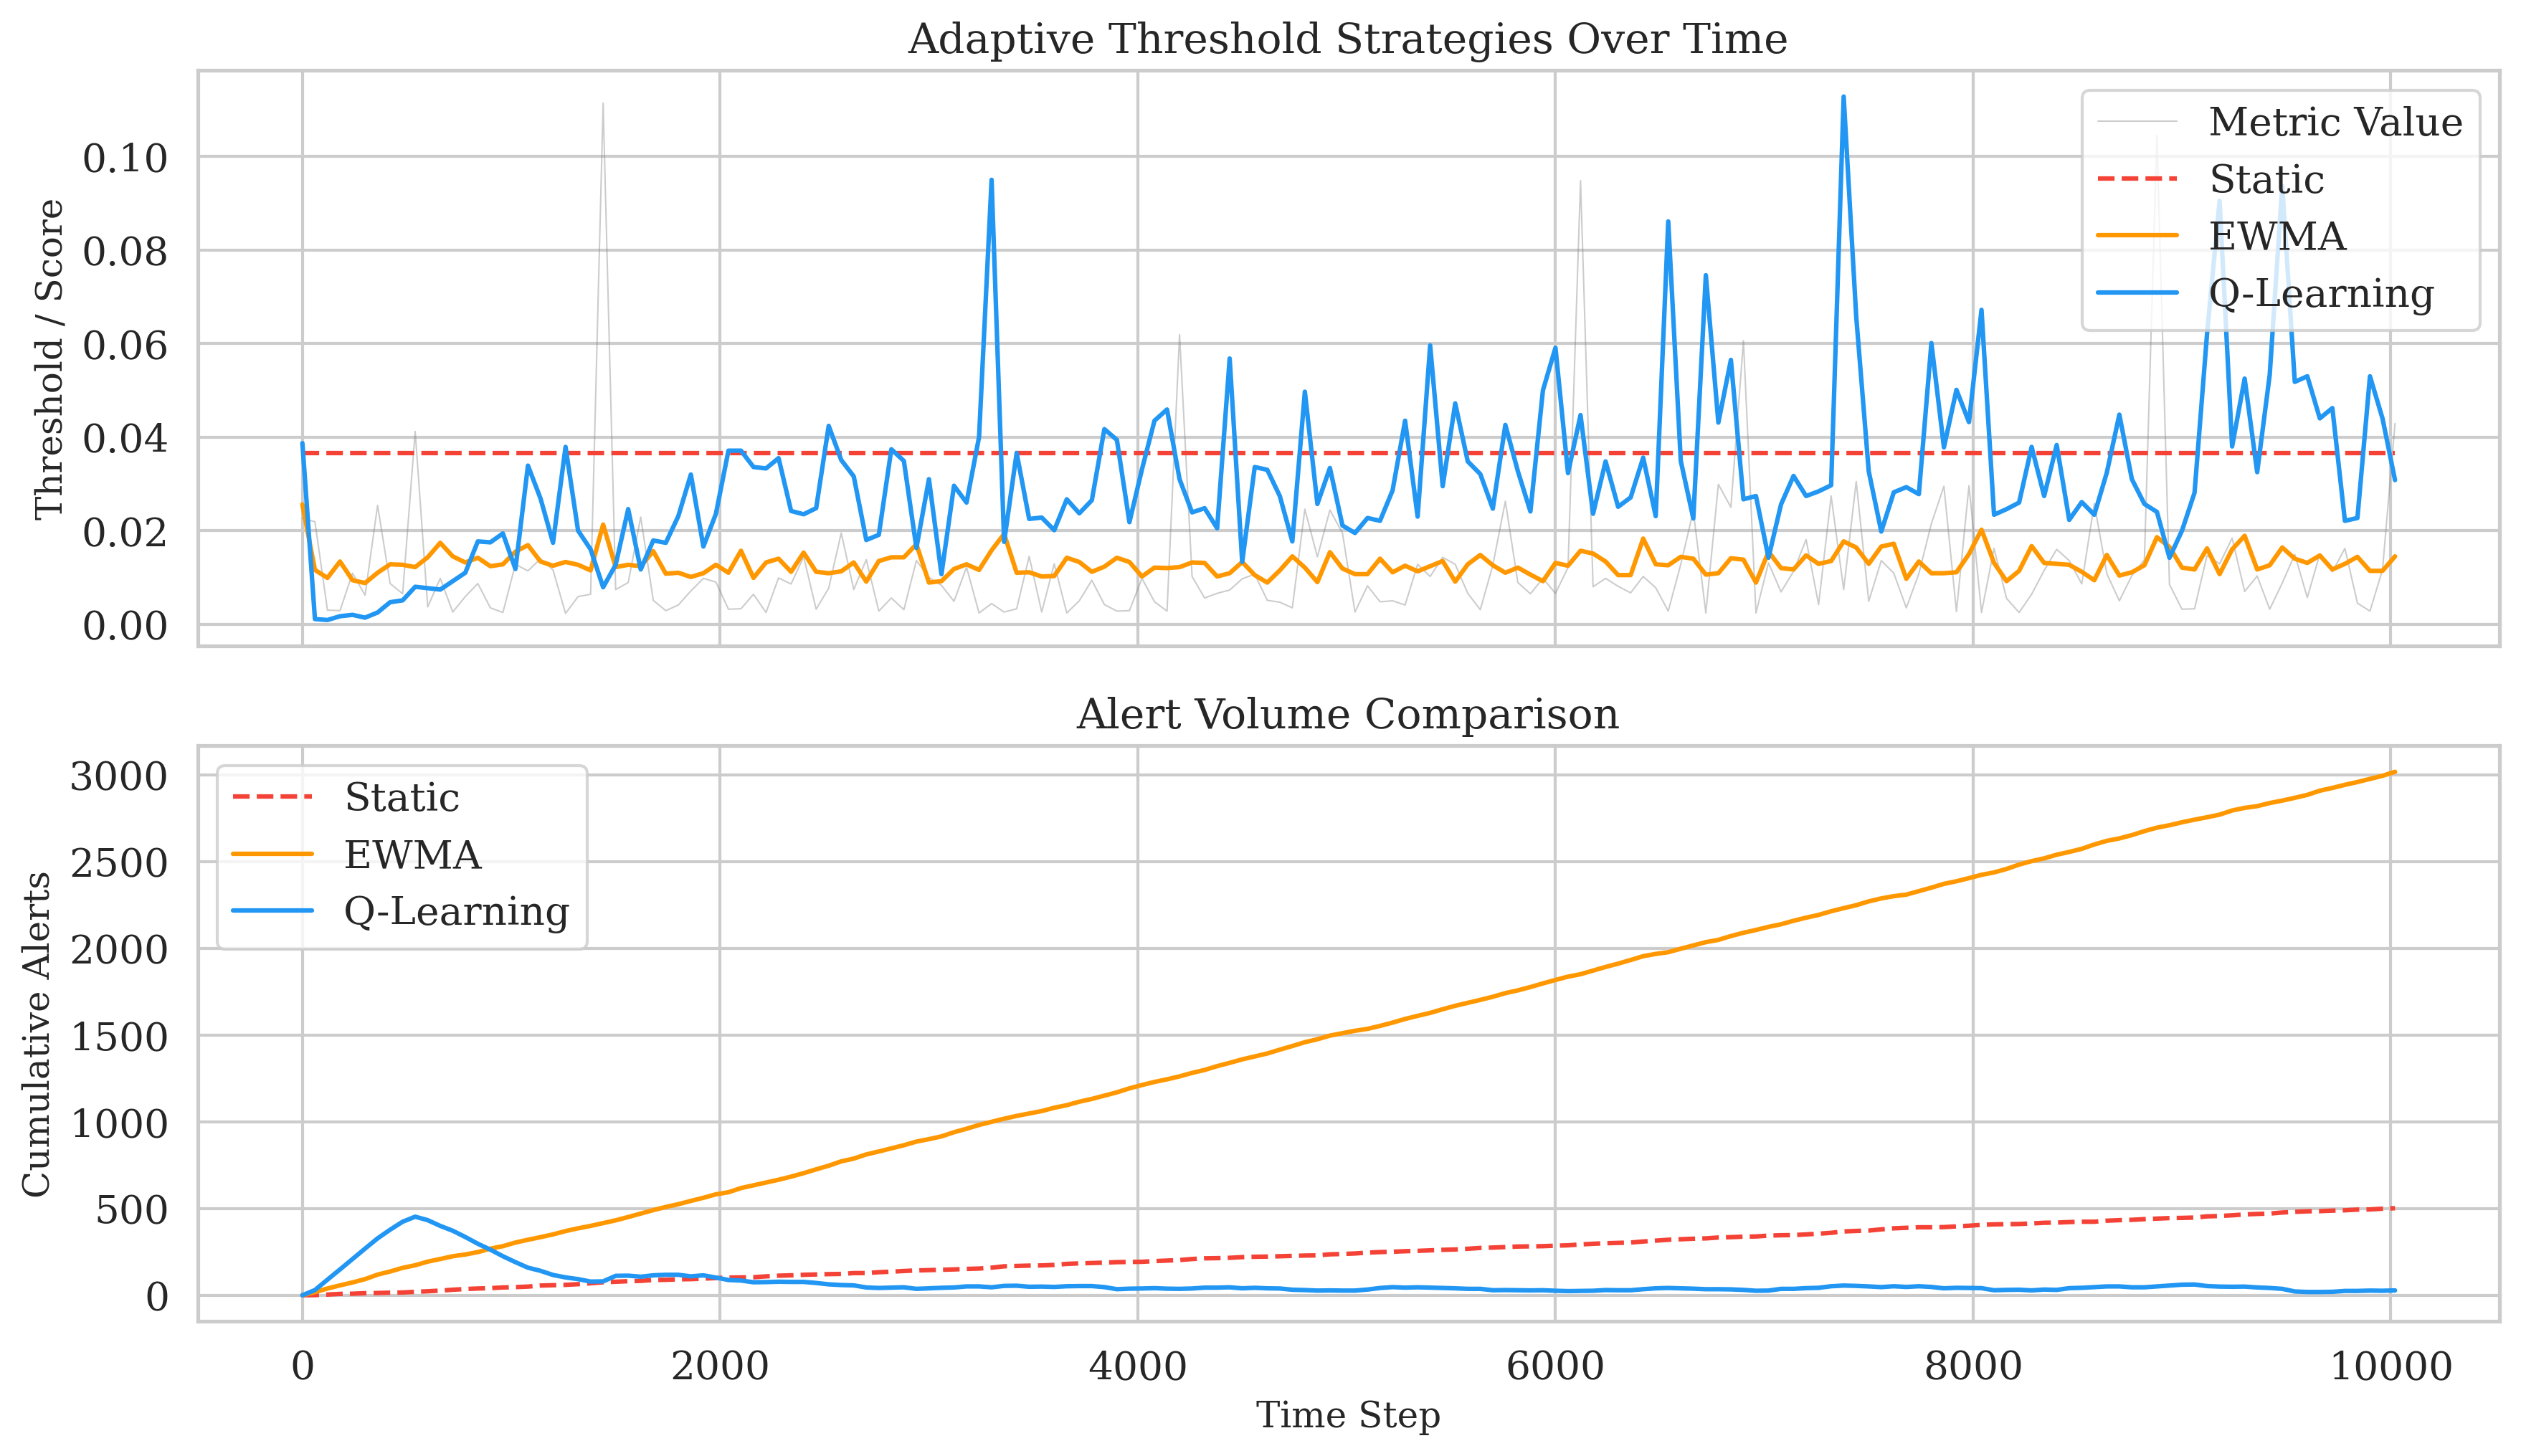
\includegraphics[width=0.90\textwidth]{chapters/06_experimental_evaluation/assets/adaptive_threshold.png}
    \caption{Threshold trajectories and cumulative alerts (seed~42). The static
             threshold (blue) accumulates alerts linearly. EWMA (orange)
             over-triggers due to its smoothing lag. Q-learning (green)
             initially over-alerts during $\varepsilon$-greedy exploration,
             then stabilizes after the exploration rate decays below 0.05.}
    \label{fig:adaptive_threshold}
\end{figure}

The Q-learning evaluation (10\,020-minute SMD stream, seed~42) is exploratory
rather than production-ready. Early exploration is unstable: by minute~360 it
produces 328 alerts and FPR~$=$~0.908. After a longer horizon, however, the
learned threshold stabilizes. At the final logged point it produces 28~alerts,
FPR~$=$~0.0155, and F1~$=$~0.5526, compared with 502 static-threshold alerts
and 3\,018 EWMA alerts.

\subsection{Q-Learning Convergence Analysis}
\label{subsec:eval_threshold_convergence}

\begin{table}[H]
    \centering
    \small
    \begin{tabular}{|c|c|c|c|c|}
        \hline
        \textbf{Min} & \textbf{$\tau_t$} & \textbf{$\varepsilon$}
        & \textbf{Reward} & \textbf{F1} \\
        \hline
        0 & 0.0387 & 0.0995 & -5.0 & 0.000 \\
        360 & 0.0025 & 0.0831 & -1470.1 & 0.136 \\
        1380 & 0.0160 & 0.0498 & -2655.9 & 0.646 \\
        5040 & 0.0195 & 0.0100 & -3715.3 & 0.575 \\
        10020 & 0.0308 & 0.0100 & -5057.5 & 0.553 \\
        \hline
    \end{tabular}
    \caption{Q-learning state evolution (seed~42). The $\varepsilon$-decay
             from 0.10 to 0.01 confirms the exploration-to-exploitation
             transition. The persistently negative cumulative reward
             indicates that the default reward coefficients penalize early
             exploration too heavily; warm-starting or reward shaping would
             mitigate this.}
    \label{tab:ql_convergence}
\end{table}

The $\varepsilon$-decay from 0.10 to 0.01 confirms the expected
exploration-to-exploitation transition, but the cumulative reward remains
negative. The threshold policy therefore learns a useful final alert volume only
after a costly exploration phase. This makes the current tabular policy a
diagnostic result: it demonstrates that adaptive thresholding can reduce alert
fatigue, but also that reward shaping and warm starts are necessary before
deployment.

% ============================================================================
\section{Scalability}
\label{sec:eval_scalability}

\begin{table}[H]
    \centering
    \small
    \begin{tabular}{|r|r|r|}
        \hline
        \textbf{Nodes} & \textbf{Aggr.\,(ms)} & \textbf{Mem\,$\Delta$\,(MB)} \\
        \hline
        5 & 5.1 & 4.0 \\
        50 & 48.3 & 25.1 \\
        100 & 75.7 & 50.1 \\
        500 & 508.2 & 21.8 \\
        1\,000 & 990.1 & 42.3 \\
        \hline
    \end{tabular}
    \caption{FedAvg aggregation scalability up to 1\,000 participants.}
    \label{tab:scalability}
\end{table}

\begin{figure}[H]
    \centering
    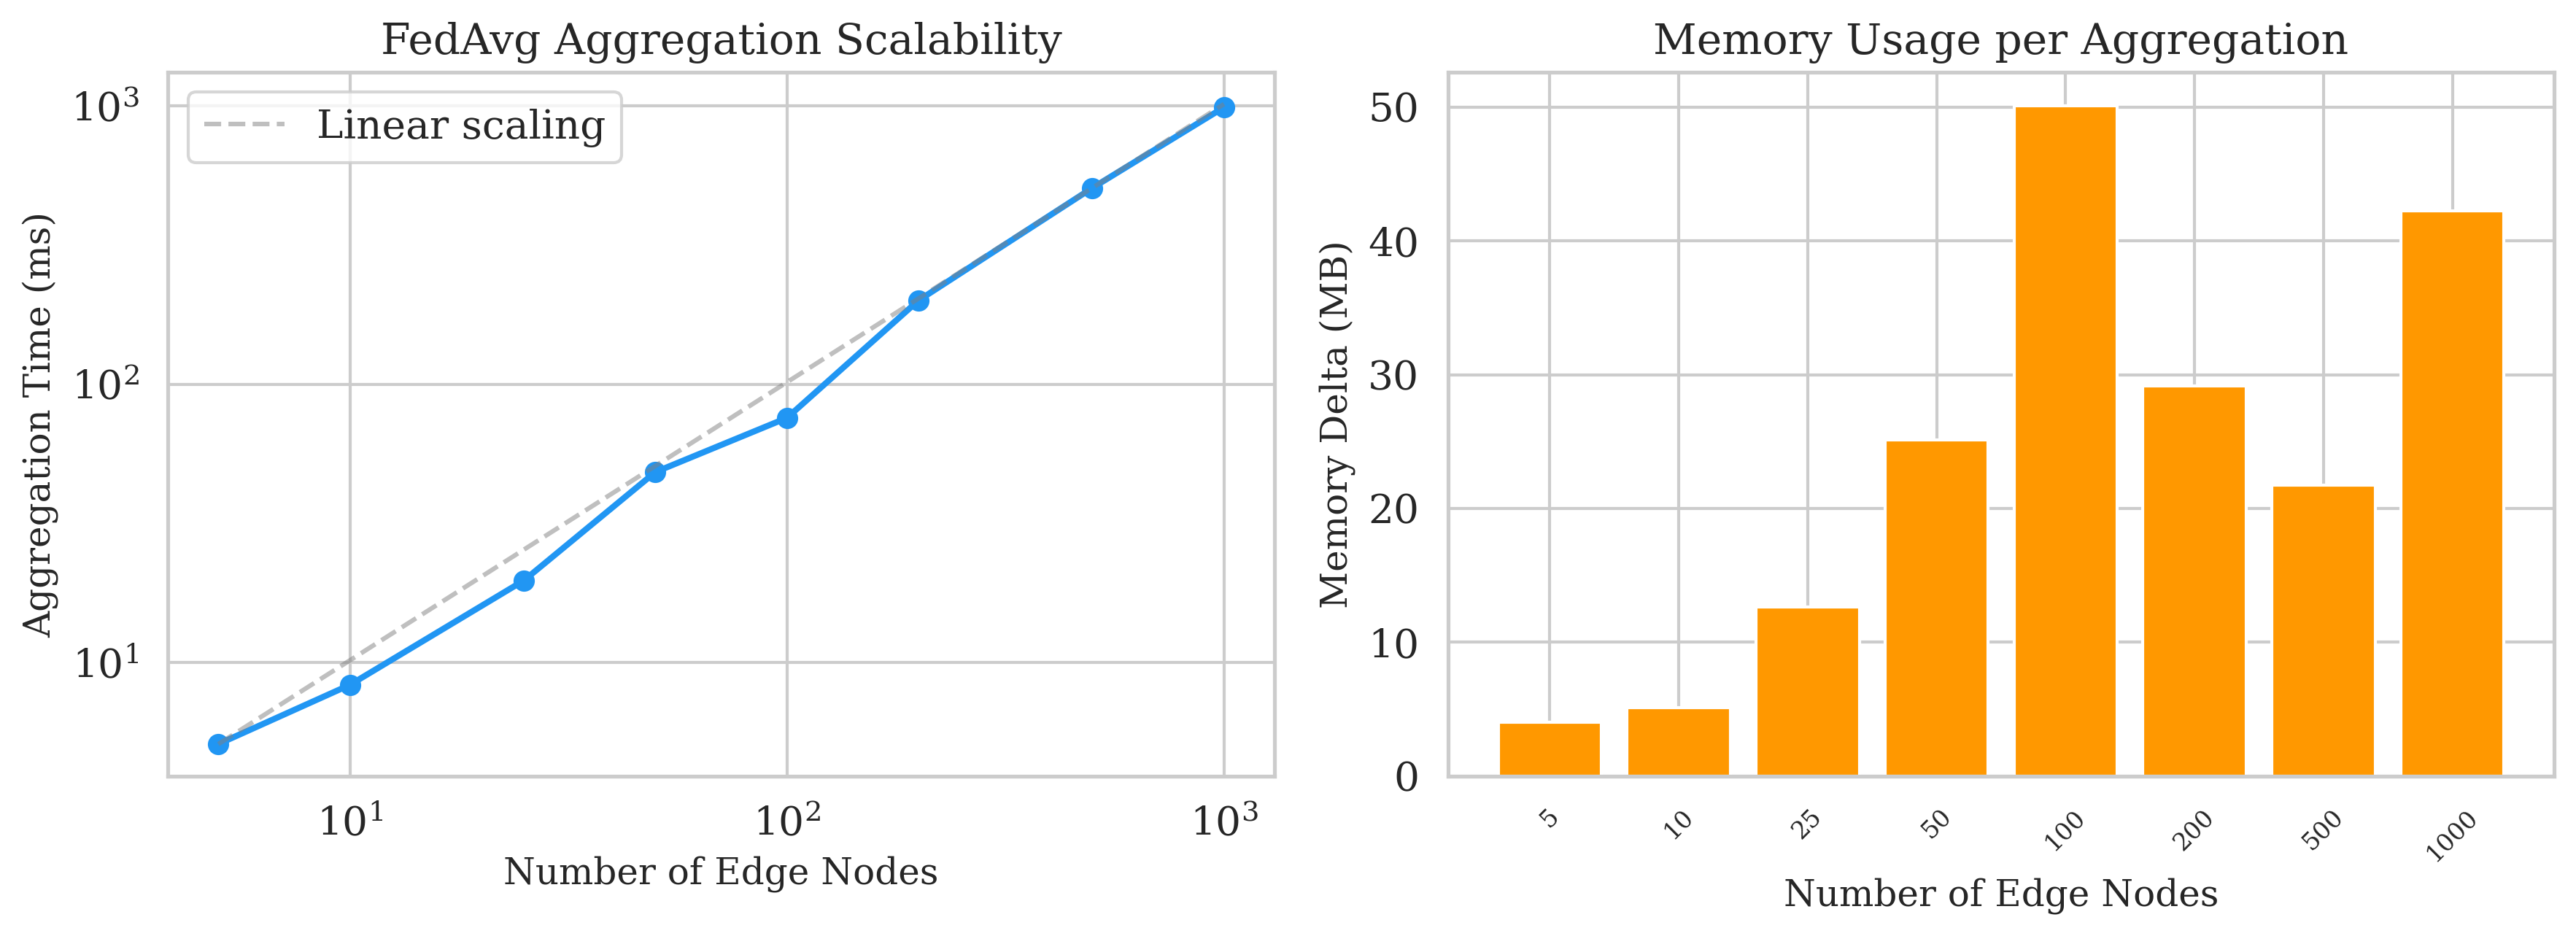
\includegraphics[width=0.85\textwidth]{chapters/06_experimental_evaluation/assets/scalability.png}
    \caption{FedAvg aggregation time and memory vs.\ client count; both
             scale linearly, confirming the coordinator is not the bottleneck.
             Clients are simulated in-process; network latency was not emulated.}
    \label{fig:scalability}
\end{figure}

\subsection{Ablation Summary}
\label{subsec:eval_ablation}

The component comparisons show the incremental role of each subsystem: the
LSTM-AE replaces the failed static baseline with the detection results in
Table~\ref{tab:detection_results};
FedAvg improves over the centralized model; DP-SGD preserves
utility for mild noise; compression reduces communication without altering
model semantics; RCA reaches 89\% Top-3 on Train-Ticket; and Q-learning
contributes an exploratory threshold-control result.

% ============================================================================
\section{Threats to Validity}
\label{sec:eval_validity}

\textbf{Dataset representativeness.} SMD provides real server telemetry but
does not cover application-level signals, deployment events, or log-derived
features found in production microservice platforms.

\textbf{Synthetic anomaly injection.} Injected CPU spikes, memory leaks, and
latency surges provide controlled labels, but synthetic faults may be cleaner
than real incidents with overlapping failures and operator interventions.

\textbf{Single-workstation execution.} Running on one CPU-only machine keeps
comparisons reproducible but underestimates heterogeneity in edge deployments.
The scalability experiment isolates aggregation cost but does not emulate
wide-area network behavior.

\textbf{Differential privacy accounting.} The $\varepsilon$ values are
approximate operating points. Tight clipping recovers utility but reduces
practical perturbation; empirical attack validation remains future work.

\textbf{Q-learning horizon.} The 10\,020-minute stream shows eventual
stabilization but does not prove robustness under workload shifts or
different anomaly rates.

% ============================================================================
\section{Discussion}
\label{sec:eval_discussion}

The results support three system-level conclusions. First, federated training is
not only privacy-preserving but also effective for this telemetry setting: the
federated LSTM-AE outperforms the centralized baseline on SMD
(\S\ref{sec:eval_detection}). Second, the DP study identifies a usable
privacy--utility region ($\sigma \leq 0.0005$) and shows that clipping is a
decisive control variable (\S\ref{subsec:eval_clipping}); tight clipping
recovers utility, but its practical privacy strength must be validated.

Third, the operational components are feasible but unevenly mature. Compression
and FedAvg introduce little overhead (\S\ref{sec:eval_fl_comm}), and RCA gives
operators a useful Top-3 candidate set on Train-Ticket
(\S\ref{sec:eval_rca}). The Q-learning threshold policy reduces final alert
volume (\S\ref{sec:eval_threshold}), but its early FPR spike and negative
cumulative reward show that the current tabular policy still needs reward
shaping and warm-starting before deployment.

\textbf{Why does the federated model outperform the centralized baseline?}
Both baselines used Config~C, the same learning rate, and seed~42. The
centralized model pools all 28~SMD machines into one dataset; the federated
model trains locally per machine before averaging. We hypothesize that SMD's
cross-machine diversity acts as implicit regularization: each local model
specializes, and FedAvg averages out local overfitting. Additionally, the
95th-percentile threshold is calibrated per-machine in the federated setting but
globally in the centralized setting, likely improving threshold fit. This
result reflects SMD's structure and should not be generalized to claim that FL
always outperforms centralized training.

\subsection{Privacy Guarantee Scope}
\label{subsec:privacy_scope}

The privacy guarantee provided in this thesis is \emph{theoretical, not
empirical}. The $\varepsilon$ values reported in Tables~\ref{tab:dp_impact}
and~\ref{tab:clip_norm} are computed via the RDP moments accountant and
represent bounds on per-sample information leakage under the assumed noise
model. They should be interpreted as formal operating points, not as
demonstrated resistance to practical attacks.

Two specific concerns apply. First, membership inference
\cite{shokri2017membership} and model inversion \cite{fredrikson2015model}
have not been tested against the trained LSTM-AE models; such tests remain the
highest-priority future experiment (\S\ref{sec:conclusion_future}). Second, the
tight-clipping result ($C{=}0.01$) recovers detection utility by reducing the
absolute perturbation $\sigma C$ by $100\times$. While the RDP accountant
reports the same $\varepsilon$ for a given $\sigma$, the practical noise
injected into the model update is far smaller, which may weaken resistance to
reconstruction-based attacks. Until empirical attack validation is performed,
the privacy claim should be read as a formal bound, not as a deployment-ready
guarantee.
